\documentclass[11pt,a4paper]{article}

% Image mode: pdf.
% Image paths stay relative. In PDF mode, place same-basename PDF conversions
% of the chapter SVG files in the assets/ directory beside this source.

\usepackage{iftex}
\ifPDFTeX
  \PackageError{handout}{This template requires XeTeX or Tectonic}{Compile with xelatex or tectonic.}
\fi

\usepackage[a4paper,top=18mm,bottom=20mm,left=20mm,right=20mm,headsep=6mm]{geometry}
\usepackage{fontspec}
\usepackage{xeCJK}
\usepackage{amsmath}
\usepackage{unicode-math}

% Font settings are intentionally visible in the generated .tex file.
% These defaults target the macOS machine used for the released PDF.
% Change the family names when compiling on another system.
\setmainfont{Songti TC}
\setsansfont{Heiti TC}
\setmonofont{Menlo}
\setCJKmainfont{Songti TC}
\setCJKsansfont{Heiti TC}
\setCJKmonofont{Heiti TC}
\setmathfont{STIX Two Math}
\XeTeXlinebreaklocale "zh"
\XeTeXlinebreakskip=0pt plus 1pt

\usepackage{xcolor}
\definecolor{HandoutBlue}{HTML}{215A91}
\definecolor{HandoutBlueLight}{HTML}{EEF5FC}
\definecolor{HandoutGreen}{HTML}{39715A}
\definecolor{HandoutGreenLight}{HTML}{EFF8F3}
\definecolor{HandoutGold}{HTML}{8A641C}
\definecolor{HandoutGoldLight}{HTML}{FFF8E8}
\definecolor{HandoutInk}{HTML}{253142}
\definecolor{HandoutMuted}{HTML}{667085}

\usepackage{graphicx}
\makeatletter
% Pandoc 3 emits an accessibility `alt` key for raster/PDF images. Older
% graphicx releases do not know that key, so accept it without changing layout.
\@ifundefined{KV@Gin@alt}{\define@key{Gin}{alt}{}}{}
\newsavebox\pandoc@box
\newcommand*\pandocbounded[1]{%
  \sbox\pandoc@box{#1}%
  \Gscale@div\@tempa{\textheight}{\dimexpr\ht\pandoc@box+\dp\pandoc@box\relax}%
  \Gscale@div\@tempb{\linewidth}{\wd\pandoc@box}%
  \ifdim\@tempb\p@<\@tempa\p@\let\@tempa\@tempb\fi
  \ifdim\@tempa\p@<\p@\scalebox{\@tempa}{\usebox\pandoc@box}%
  \else\usebox{\pandoc@box}%
  \fi
}
\makeatother
\usepackage{float}
\floatplacement{figure}{H}
% Pandoc uses LTcaptype=none for uncaptioned longtables. The caption package
% expects that name to exist as a counter even though it is never displayed.
\newcounter{none}
\usepackage{caption}
\captionsetup[figure]{labelformat=empty,labelsep=none,font=small}

\usepackage{booktabs,longtable,array,calc}
\usepackage{etoolbox}
\makeatletter
\patchcmd\longtable{\par}{\if@noskipsec\mbox{}\fi\par}{}{}
\makeatother

\usepackage[most]{tcolorbox}
\tcbuselibrary{breakable,skins}
\newtcolorbox{HandoutLearningMap}{
  enhanced,breakable,colback=HandoutBlueLight,colframe=HandoutBlue,
  boxrule=0.8pt,arc=1.5mm,left=3mm,right=3mm,top=2mm,bottom=2mm,
  before skip=8pt,after skip=10pt
}
\newtcolorbox{HandoutWorkedExample}{
  enhanced,breakable,colback=HandoutGreenLight,colframe=HandoutGreen,
  boxrule=0.65pt,arc=1.5mm,left=3mm,right=3mm,top=2mm,bottom=2mm,
  before skip=8pt,after skip=10pt
}
\newtcolorbox{HandoutSelfCheck}{
  enhanced,breakable,colback=HandoutGoldLight,colframe=HandoutGold,
  boxrule=0.65pt,arc=1.5mm,left=3mm,right=3mm,top=2mm,bottom=2mm,
  before skip=8pt,after skip=10pt
}

\usepackage{titlesec}
\titleformat{\section}{\sffamily\bfseries\Large\color{HandoutBlue}}{}{0pt}{}
\titleformat{\subsection}{\sffamily\bfseries\large\color{HandoutInk}}{}{0pt}{}
\titleformat{\subsubsection}{\sffamily\bfseries\normalsize\color{HandoutInk}}{}{0pt}{}
\titlespacing*{\section}{0pt}{1.4em}{0.55em}
\titlespacing*{\subsection}{0pt}{1.15em}{0.45em}
\titlespacing*{\subsubsection}{0pt}{0.9em}{0.35em}
\setcounter{secnumdepth}{-\maxdimen}

\usepackage{hyperref}
\usepackage{bookmark}
\IfFileExists{xurl.sty}{\usepackage{xurl}}{}
\urlstyle{same}
\hypersetup{
  colorlinks=true,
  linkcolor=HandoutBlue,
  urlcolor=HandoutBlue,
  citecolor=HandoutBlue,
  pdftitle={選化II-3 化學反應速率},
  pdfsubject={化學},
  pdfcreator={Pandoc with the HighSchooContent LaTeX template}
}

\setlength{\parindent}{0pt}
\setlength{\parskip}{0.55em plus 0.15em minus 0.1em}
\setlength{\emergencystretch}{3em}
\setlength{\LTpre}{0.5em}
\setlength{\LTpost}{0.5em}
\renewcommand{\arraystretch}{1.18}
\providecommand{\tightlist}{%
  \setlength{\itemsep}{0pt}\setlength{\parskip}{0pt}}
\pagestyle{plain}


\begin{document}

\begin{tcolorbox}[
  enhanced,colback=white,colframe=HandoutBlue,boxrule=1.1pt,arc=2mm,
  borderline west={3pt}{0pt}{HandoutBlue},left=5mm,right=4mm,top=4mm,bottom=4mm
]
{\sffamily\small\bfseries\color{HandoutBlue}學生講義}\par
{\sffamily\bfseries\LARGE\color{HandoutInk}選化II-3 化學反應速率}\par
\vspace{0.35em}{\large 由濃度---時間資料建立速率定律，再用碰撞、能障與反應機構解釋濃度、溫度、接觸面積與催化劑的影響}\par
\vspace{0.45em}{\small\color{HandoutMuted}%
科目：化學
\quad 課程：普通高中選修化學 II
\quad 版本：學生版｜核心＋理解
\quad 校訂：2026-08-29
}\par
\vspace{0.25em}{\small\color{HandoutMuted}範圍：現行選修化學 II 第三章主線；涵蓋反應速率與測量、速率定律、零級與一級反應、碰撞理論、活化能與反應機構、影響速率的因素及碘鐘反應實驗}\par
\end{tcolorbox}


同一個反應可以在數秒內完成，也可以持續數年。速率學把「變化快慢」轉成可測量的濃度---時間關係，再由實驗決定速率定律。碰撞理論、能障與反應機構提供微觀解釋，使我們能推測何種操作可以加快或減慢反應。食品冷藏、藥品安定性、工業反應器、汽車觸媒轉化器與生化酵素都直接使用這些模型。

\begin{HandoutLearningMap}

\subsection{本章問題與能力}\label{ux672cux7ae0ux554fux984cux8207ux80fdux529b}

\begin{enumerate}
\def\labelenumi{\arabic{enumi}.}
\tightlist
\item
  如何由濃度---時間圖求平均速率、瞬時速率與初速率？
\item
  化學計量係數如何把各物種的濃度變化轉成同一個反應速率？
\item
  如何由初速率資料求反應級數、速率常數與其單位？
\item
  零級與一級反應的濃度---時間式、線性圖與半生期有何特徵？
\item
  有效碰撞、活化能、活化複合體與速率常數如何連結？
\item
  如何由多步反應辨認中間體、催化劑與速率決定步驟？
\item
  反應物本質、濃度、接觸面積、溫度與催化劑如何改變反應速率？
\item
  如何以碘鐘反應設計控制變因實驗，並區分觀察值與模型推論？
\end{enumerate}

\end{HandoutLearningMap}

\section{1. 反應速率}\label{ux53cdux61c9ux901fux7387}

\subsection{1.1 反應速率的定義與測量}\label{ux53cdux61c9ux901fux7387ux7684ux5b9aux7fa9ux8207ux6e2cux91cf}

對物質 \(A\) 而言，某時段的平均濃度變化率為

\[
\frac{\Delta[A]}{\Delta t}
=\frac{[A]_{t_2}-[A]_{t_1}}{t_2-t_1}.
\]

反應物濃度隨時間下降，\(\Delta[A]/\Delta t<0\)；生成物濃度隨時間上升，\(\Delta[P]/\Delta t>0\)。反應速率通常以正值表示，因此反應物的定義前加負號：

\[
\text{反應物的平均消耗速率}
=-\frac{\Delta[A]}{\Delta t},
\qquad
\text{生成物的平均生成速率}
=\frac{\Delta[P]}{\Delta t}.
\]

濃度常用 \(\mathrm{mol\,L^{-1}}\) 或 M，時間常用 s，因此濃度速率的常用單位為 \(\mathrm{M\,s^{-1}}\)。若實驗以質量、氣體體積、壓力或吸光值追蹤反應，可以直接報告該觀測量的變化率；當測得量與濃度的比例關係已經校正，便可換算為濃度速率。

\begin{figure}
\centering
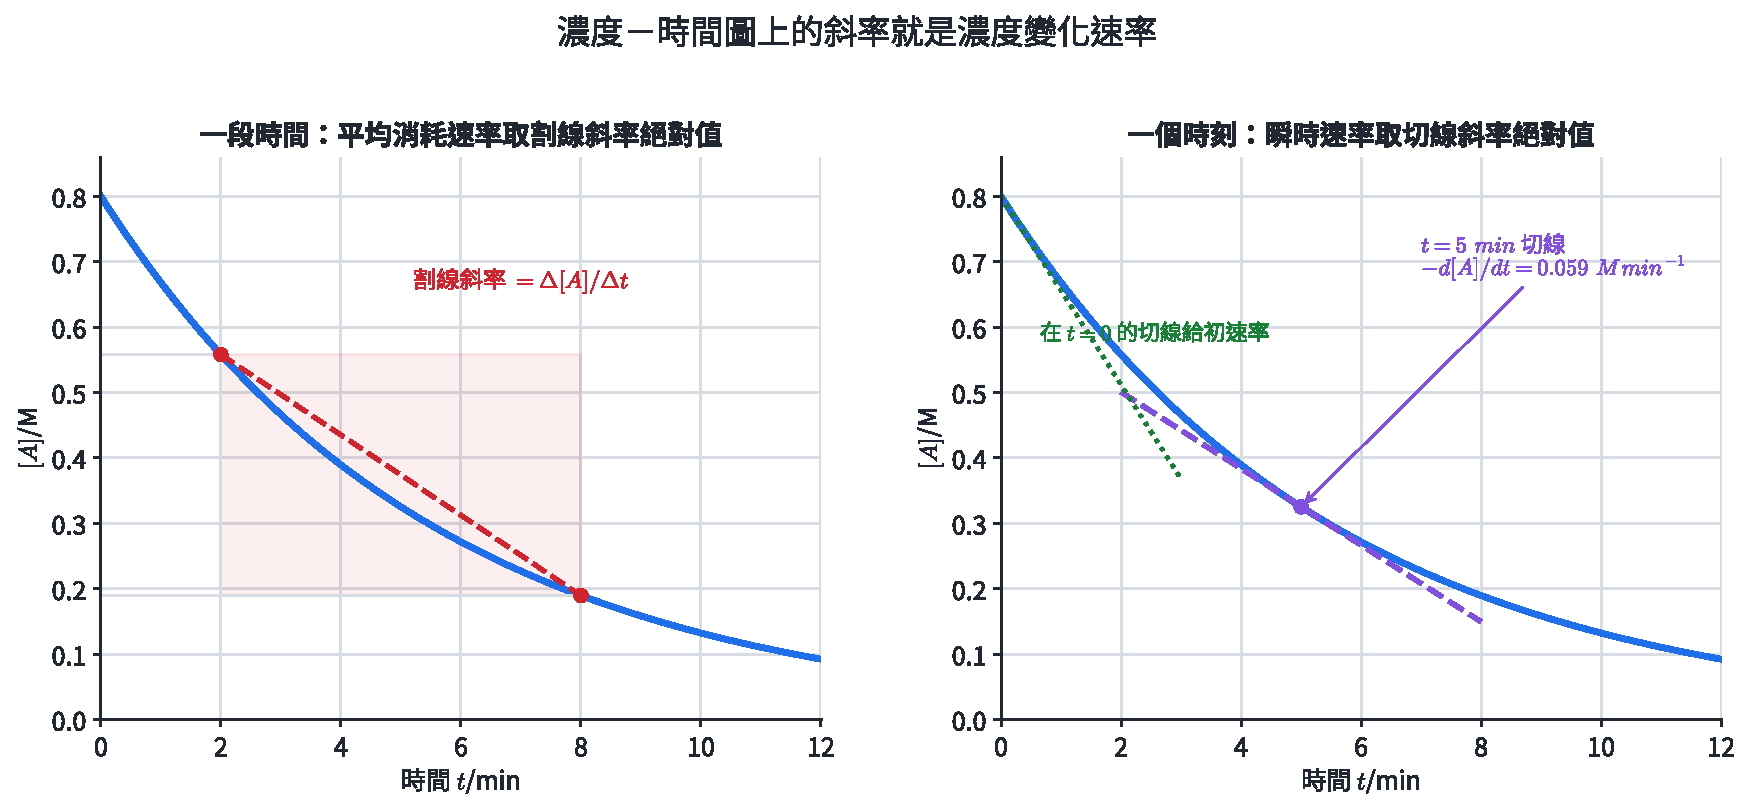
\includegraphics[width=0.98\linewidth,height=\textheight,keepaspectratio,alt={圖 1｜左圖以兩端點連成割線求時段平均速率；右圖以指定時刻的切線斜率求瞬時速率。}]{assets/選化II-3-濃度時間與速率斜率.pdf}
\caption{圖 1｜左圖以兩端點連成割線求時段平均速率；右圖以指定時刻的切線斜率求瞬時速率。}
\end{figure}

圖 1 建立三種速率：

\begin{itemize}
\tightlist
\item
  \textbf{平均速率}：濃度---時間圖在 \(t_1\) 與 \(t_2\) 之間的割線斜率絕對值。
\item
  \textbf{瞬時速率}：濃度---時間圖在某時刻的切線斜率絕對值。反應物 \(A\) 的瞬時消耗速率為 \(-\mathrm d[A]/\mathrm dt\)。
\item
  \textbf{初速率 \(r_0\)}：\(t=0\) 時的瞬時速率。此時生成物尚少、逆反應影響小，適合用來求速率定律。
\end{itemize}

在大多數反應中，反應物濃度隨時間下降，有效碰撞機會也降低，因此曲線逐漸變平。這也說明同一反應在不同時段的平均速率通常不同。

\subsection{1.2 化學計量係數與反應速率}\label{ux5316ux5b78ux8a08ux91cfux4fc2ux6578ux8207ux53cdux61c9ux901fux7387}

對反應

\[
aA+bB\longrightarrow cC+dD,
\]

同一段時間內的物質量變化依反應係數成比。以係數除去各物種的濃度變化，可得相同的反應速率：

\[
r=-\frac{1}{a}\frac{\Delta[A]}{\Delta t}
  =-\frac{1}{b}\frac{\Delta[B]}{\Delta t}
  = \frac{1}{c}\frac{\Delta[C]}{\Delta t}
  = \frac{1}{d}\frac{\Delta[D]}{\Delta t}.
\]

\begin{figure}
\centering
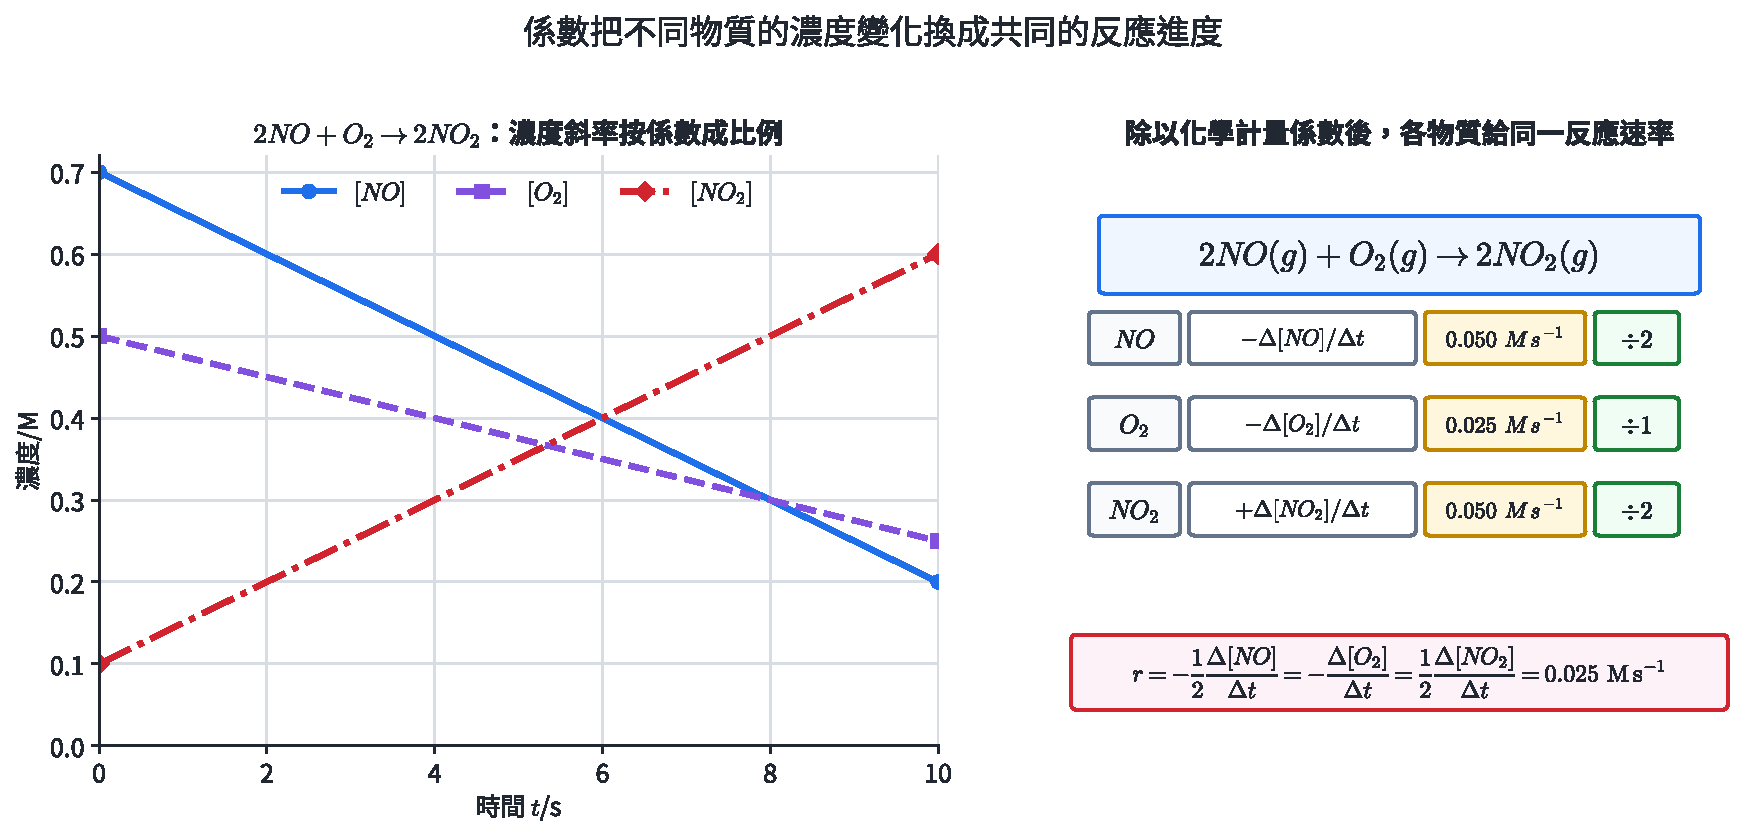
\includegraphics[width=0.98\linewidth,height=\textheight,keepaspectratio,alt={圖 2｜在 2NO+O\_2\textbackslash rightarrow2NO\_2 中，NO 與 NO\_2 的濃度斜率大小是 O\_2 的兩倍；以係數歸一後皆得到同一個 r。}]{assets/選化II-3-化學計量速率關係.pdf}
\caption{圖 2｜在 \(2NO+O_2\rightarrow2NO_2\) 中，\(NO\) 與 \(NO_2\) 的濃度斜率大小是 \(O_2\) 的兩倍；以係數歸一後皆得到同一個 \(r\)。}
\end{figure}

係數歸一化的用途是使「反應速率」不依賴所選物種。若題目問「\(O_2\) 的消耗速率」，就直接給 \(-\Delta[O_2]/\Delta t\)；若問「該反應的速率 \(r\)」，則依係數歸一化。這個字眼差異會改變數值，是作答時必須明確的條件。

\begin{HandoutWorkedExample}

\subsection{示範 1｜平均消耗速率與生成速率}\label{ux793aux7bc4-1ux5e73ux5747ux6d88ux8017ux901fux7387ux8207ux751fux6210ux901fux7387}

反應 \(2N_2O_5(g)\rightarrow4NO_2(g)+O_2(g)\) 進行 \(40.0\ \mathrm{s}\) 後，\([N_2O_5]\) 由 \(0.640\ \mathrm M\) 降為 \(0.520\ \mathrm M\)。求 \(N_2O_5\) 的平均消耗速率、\(NO_2\) 的平均生成速率與歸一化反應速率 \(r\)。

\[
\Delta[N_2O_5]=0.520-0.640=-0.120\ \mathrm M,
\]

\[
-\frac{\Delta[N_2O_5]}{\Delta t}
=-\frac{-0.120}{40.0}
=3.00\times10^{-3}\ \mathrm{M\,s^{-1}}.
\]

由係數 \(2:4\)，

\[
\frac{\Delta[NO_2]}{\Delta t}
=\frac{4}{2}\left(3.00\times10^{-3}\right)
=6.00\times10^{-3}\ \mathrm{M\,s^{-1}}.
\]

歸一化的反應速率為

\[
r=-\frac12\frac{\Delta[N_2O_5]}{\Delta t}
=1.50\times10^{-3}\ \mathrm{M\,s^{-1}}.
\]

\(NO_2\) 的生成速率是 \(N_2O_5\) 消耗速率的兩倍，符合係數 \(4:2\)。

\end{HandoutWorkedExample}

\begin{HandoutWorkedExample}

\subsection{示範 2｜由濃度---時間資料估計瞬時速率}\label{ux793aux7bc4-2ux7531ux6fc3ux5ea6ux6642ux9593ux8cc7ux6599ux4f30ux8a08ux77acux6642ux901fux7387}

某反應中 \(A\) 的濃度資料為：

{\def\LTcaptype{none} % do not increment counter
\begin{longtable}[]{@{}rrrr@{}}
\toprule\noalign{}
\(t/\mathrm s\) & 18.0 & 20.0 & 22.0 \\
\midrule\noalign{}
\endhead
\bottomrule\noalign{}
\endlastfoot
\([A]/\mathrm M\) & 0.462 & 0.430 & 0.401 \\
\end{longtable}
}

以 \(t=20.0\ \mathrm s\) 左右對稱的割線估計當時的瞬時消耗速率。兩點割線可近似當地切線：

\[
\left.\frac{\mathrm d[A]}{\mathrm dt}\right|_{20\mathrm s}
\approx\frac{0.401-0.462}{22.0-18.0}
=-1.525\times10^{-2}\ \mathrm{M\,s^{-1}}.
\]

因此 \(A\) 的瞬時消耗速率約為 \(1.53\times10^{-2}\ \mathrm{M\,s^{-1}}\)。估計區間為 \(18.0\) 至 \(22.0\ \mathrm s\)；縮小取樣間隔通常可使結果更接近真正切線斜率。

\end{HandoutWorkedExample}

\subsection{1.3 速率定律、反應級數與速率常數}\label{ux901fux7387ux5b9aux5f8bux53cdux61c9ux7d1aux6578ux8207ux901fux7387ux5e38ux6578}

在溫度與其他條件固定時，實驗常可將初速率寫成

\[
r_0=k[A]_0^m[B]_0^n.
\]

\begin{itemize}
\tightlist
\item
  \(m\) 與 \(n\) 是各反應物的\textbf{反應級數}，由實驗決定。
\item
  \(m+n\) 是總反應級數。
\item
  \(k\) 是\textbf{速率常數}，對同一反應而言會隨溫度、催化途徑與反應介質改變。
\end{itemize}

一般總反應的速率定律指數必須由速率資料求得。只有已知為單一基本步驟的情形，速率定律才可以直接反映該步驟中的粒子數。

\begin{figure}
\centering
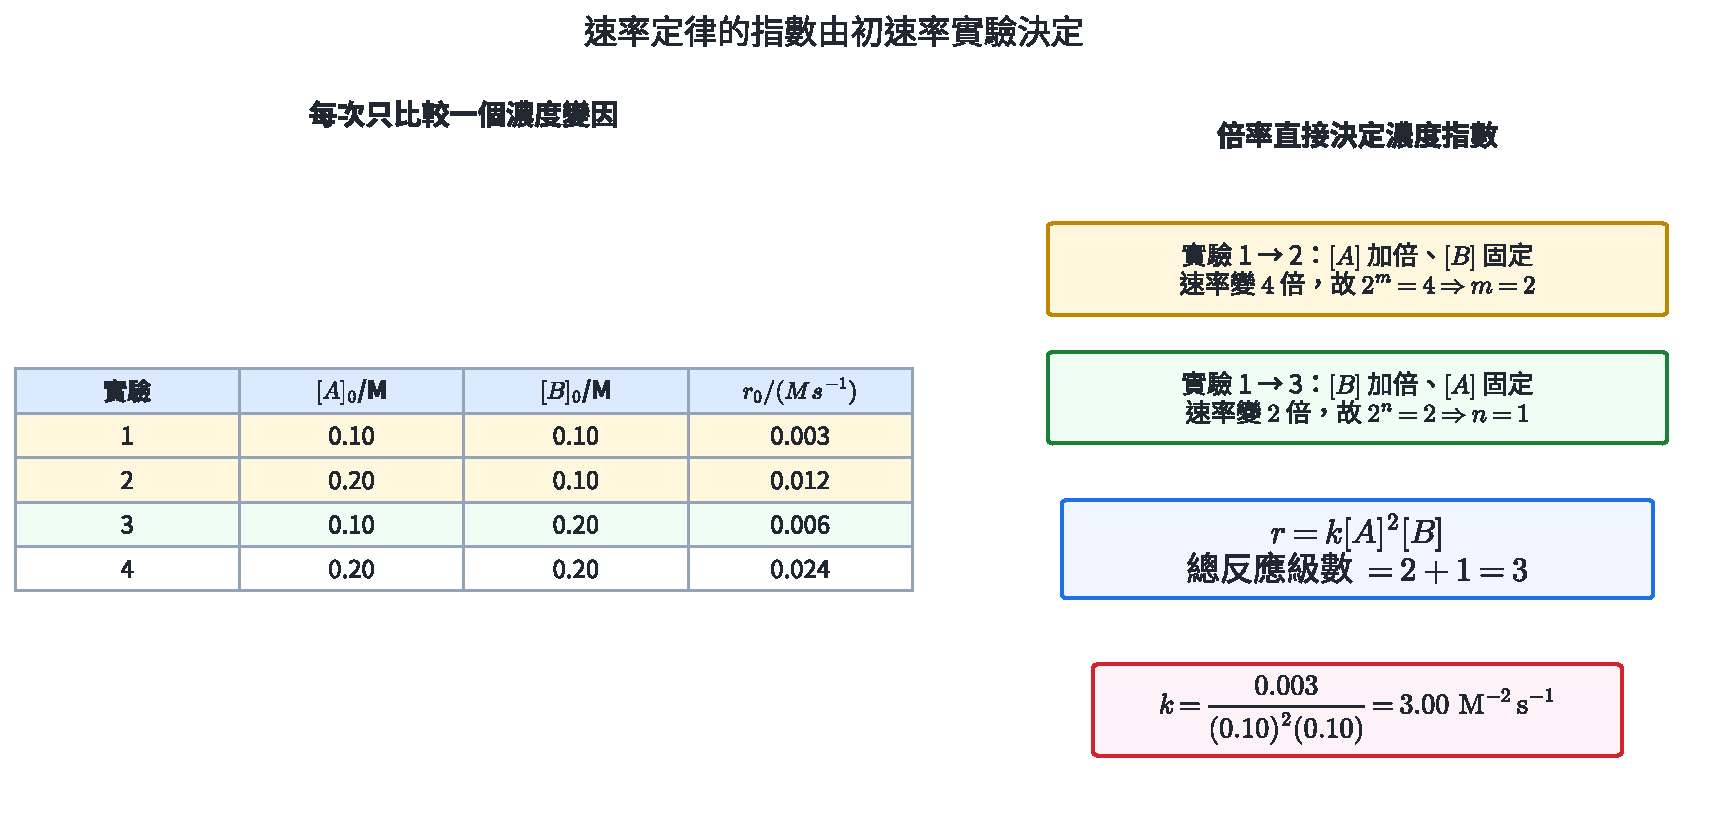
\includegraphics[width=0.97\linewidth,height=\textheight,keepaspectratio,alt={圖 3｜實驗 1→2 只加倍 A 的濃度，速率變四倍；實驗 1→3 只加倍 B 的濃度，速率變兩倍。}]{assets/選化II-3-初速率比較法.pdf}
\caption{圖 3｜實驗 1→2 只加倍 A 的濃度，速率變四倍；實驗 1→3 只加倍 B 的濃度，速率變兩倍。}
\end{figure}

比較兩組初速率實驗時，取比可以消去 \(k\) 與未改變的濃度：

\[
\frac{r_2}{r_1}
=\left(\frac{[A]_2}{[A]_1}\right)^m
 \left(\frac{[B]_2}{[B]_1}\right)^n.
\]

若其中只有 \([A]\) 改變，右式就只剩 \(([A]_2/[A]_1)^m\)。求得所有級數後，代入任一組實驗可求 \(k\)。

速率定律維度必須與速率相同。總級數為 \(N\) 時，

\[
[k]=\mathrm{M}^{\,1-N}\mathrm{s}^{-1}.
\]

{\def\LTcaptype{none} % do not increment counter
\begin{longtable}[]{@{}rr@{}}
\toprule\noalign{}
總級數 \(N\) & 速率常數單位 \\
\midrule\noalign{}
\endhead
\bottomrule\noalign{}
\endlastfoot
0 & \(\mathrm{M\,s^{-1}}\) \\
1 & \(\mathrm{s^{-1}}\) \\
2 & \(\mathrm{M^{-1}\,s^{-1}}\) \\
3 & \(\mathrm{M^{-2}\,s^{-1}}\) \\
\end{longtable}
}

\begin{HandoutWorkedExample}

\subsection{示範 3｜由初速率比較求速率定律}\label{ux793aux7bc4-3ux7531ux521dux901fux7387ux6bd4ux8f03ux6c42ux901fux7387ux5b9aux5f8b}

某反應的初速率資料為：

{\def\LTcaptype{none} % do not increment counter
\begin{longtable}[]{@{}
  >{\raggedleft\arraybackslash}p{(\linewidth - 6\tabcolsep) * \real{0.2500}}
  >{\raggedleft\arraybackslash}p{(\linewidth - 6\tabcolsep) * \real{0.2500}}
  >{\raggedleft\arraybackslash}p{(\linewidth - 6\tabcolsep) * \real{0.2500}}
  >{\raggedleft\arraybackslash}p{(\linewidth - 6\tabcolsep) * \real{0.2500}}@{}}
\toprule\noalign{}
\begin{minipage}[b]{\linewidth}\raggedleft
實驗
\end{minipage} & \begin{minipage}[b]{\linewidth}\raggedleft
\([A]_0/\mathrm M\)
\end{minipage} & \begin{minipage}[b]{\linewidth}\raggedleft
\([B]_0/\mathrm M\)
\end{minipage} & \begin{minipage}[b]{\linewidth}\raggedleft
\(r_0/(\mathrm{M\,s^{-1}})\)
\end{minipage} \\
\midrule\noalign{}
\endhead
\bottomrule\noalign{}
\endlastfoot
1 & 0.100 & 0.100 & \(3.00\times10^{-3}\) \\
2 & 0.200 & 0.100 & \(1.20\times10^{-2}\) \\
3 & 0.100 & 0.200 & \(6.00\times10^{-3}\) \\
\end{longtable}
}

設 \(r=k[A]^m[B]^n\)。實驗 1 與 2 中 \([B]\) 固定，\([A]\) 加倍，速率變四倍，故 \(4=2^m\)、\(m=2\)。實驗 1 與 3 中 \([A]\) 固定，\([B]\) 加倍，速率變兩倍，故 \(2=2^n\)、\(n=1\)。

\[
r=k[A]^2[B].
\]

代入實驗 1：

\[
k=\frac{3.00\times10^{-3}}{(0.100)^2(0.100)}
=3.00\ \mathrm{M^{-2}\,s^{-1}}.
\]

總級數為 \(3\)，所以 \(k\) 的單位 \(\mathrm{M^{-2}\,s^{-1}}\) 與維度檢查一致。

\end{HandoutWorkedExample}

\begin{HandoutWorkedExample}

\subsection{示範 4｜由速率定律預測新條件的速率}\label{ux793aux7bc4-4ux7531ux901fux7387ux5b9aux5f8bux9810ux6e2cux65b0ux689dux4ef6ux7684ux901fux7387}

已知 \(r=k[X][Y]^2\)。某條件下速率為 \(2.40\times10^{-4}\ \mathrm{M\,s^{-1}}\)。將 \([X]\) 調為原來的 \(0.50\) 倍、\([Y]\) 調為原來的 \(3.00\) 倍，溫度不變。

因 \(k\) 相同，

\[
\frac{r'}{r}=(0.50)^1(3.00)^2=4.50,
\]

\[
r'=4.50(2.40\times10^{-4})
=1.08\times10^{-3}\ \mathrm{M\,s^{-1}}.
\]

\([Y]\) 為二級，其三倍濃度貢獻九倍效果；\([X]\) 的減半使總倍率成為 \(4.50\)。

\end{HandoutWorkedExample}

\subsection{1.4 零級、一級反應與半生期}\label{ux96f6ux7d1aux4e00ux7d1aux53cdux61c9ux8207ux534aux751fux671f}

對單一反應物 \(A\) 的零級反應，

\[
-\frac{\mathrm d[A]}{\mathrm dt}=k.
\]

速率與 \([A]\) 無關，在此模型適用的濃度範圍內，積分可得

\[
[A]_t=[A]_0-kt.
\]

\([A]\) 對 \(t\) 作圖為直線，斜率 \(-k\)。令 \([A]_t=[A]_0/2\)：

\[
t_{1/2}=\frac{[A]_0}{2k}.
\]

零級半生期與初濃度成正比。由 \([A]_0\) 降到 \([A]_0/2\) 與由 \([A]_0/2\) 降到 \([A]_0/4\) 的絕對濃度變化不同，後一段只需前一段一半的時間。

對一級反應，

\[
-\frac{\mathrm d[A]}{\mathrm dt}=k[A].
\]

分離變數後由 \([A]_0\) 積分到 \([A]_t\)：

\[
\int_{[A]_0}^{[A]_t}\frac{\mathrm d[A]}{[A]}
=-k\int_0^t\mathrm dt,
\]

得

\[
\ln[A]_t=\ln[A]_0-kt,
\qquad
[A]_t=[A]_0e^{-kt}.
\]

\(\ln[A]\) 對 \(t\) 作圖為直線，斜率 \(-k\)。令 \([A]_t=[A]_0/2\)：

\[
t_{1/2}=\frac{\ln2}{k}=\frac{0.693}{k}.
\]

一級半生期與初濃度無關，每過一個半生期就保留原有量的一半。

\begin{figure}
\centering
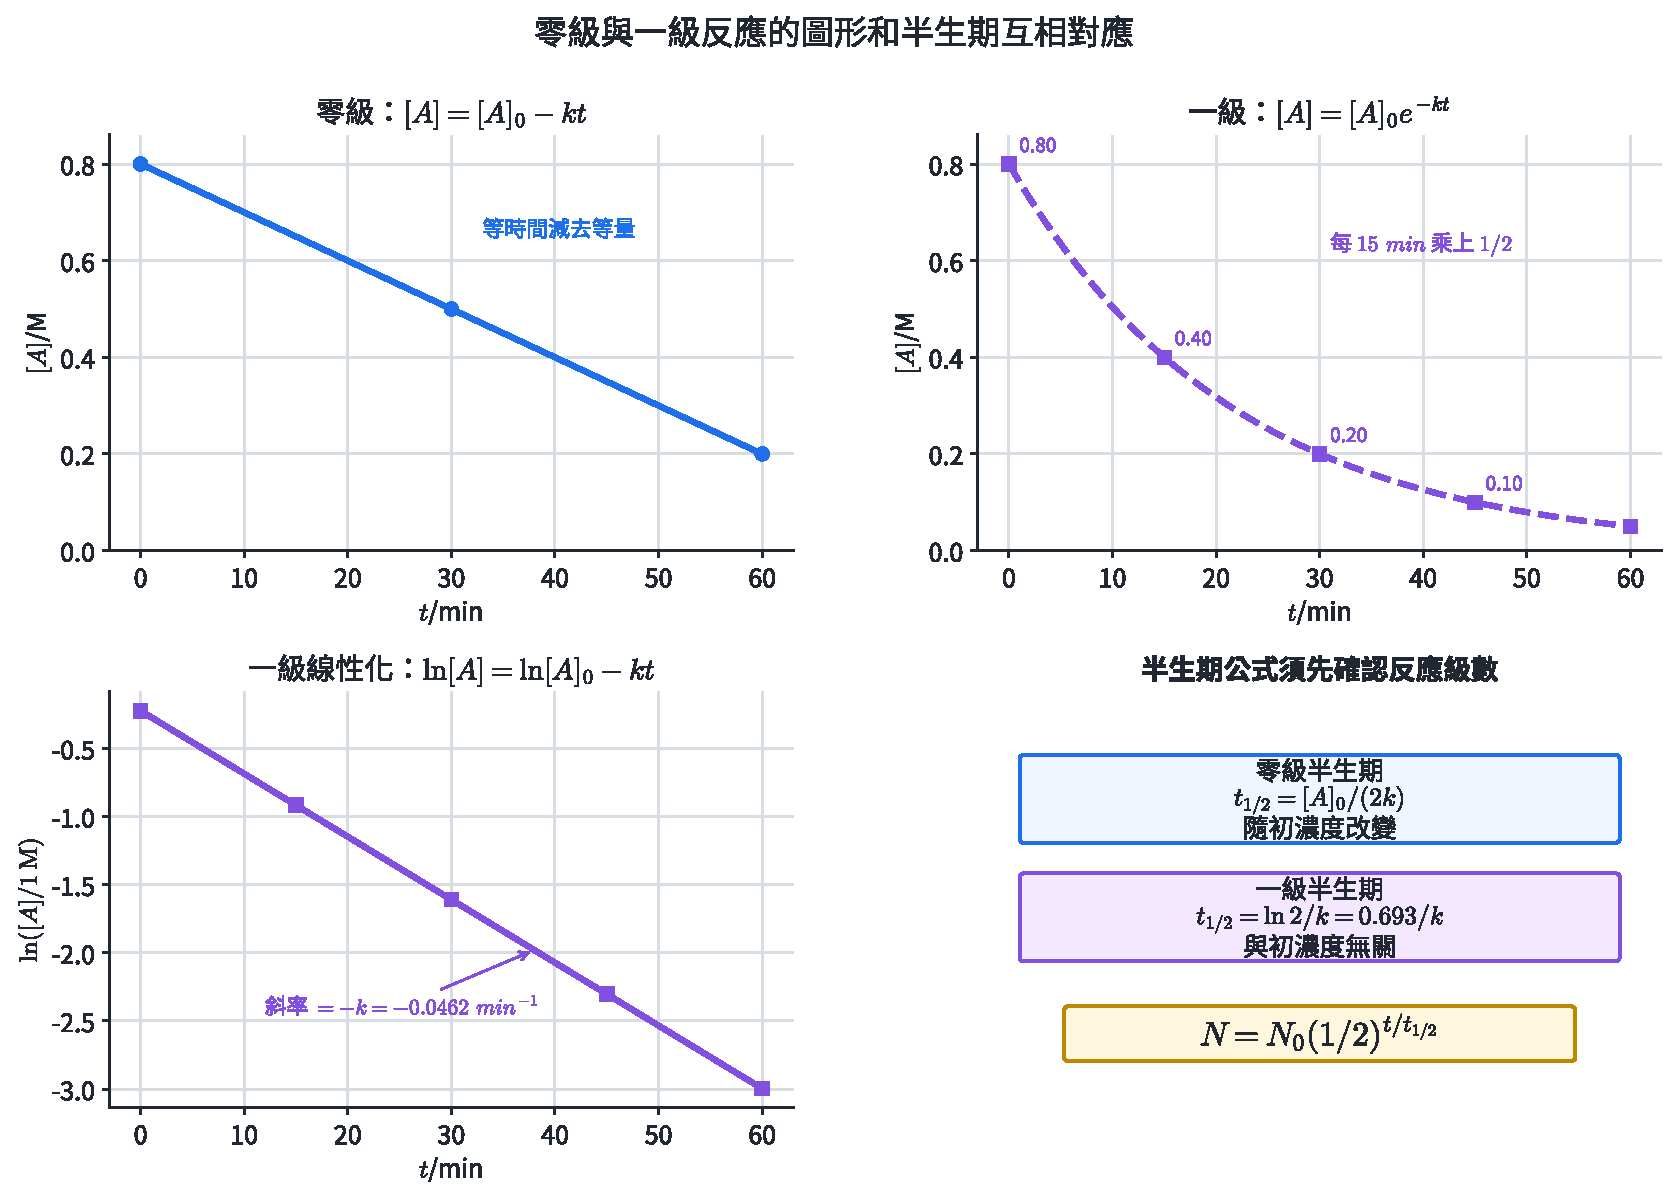
\includegraphics[width=0.96\linewidth,height=\textheight,keepaspectratio,alt={圖 4｜零級的 A 濃度線性下降，一級的 A 濃度指數下降；對應的線性圖分別是 A 濃度對 t 與其自然對數對 t。}]{assets/選化II-3-零級一級與半生期.pdf}
\caption{圖 4｜零級的 A 濃度線性下降，一級的 A 濃度指數下降；對應的線性圖分別是 A 濃度對 \(t\) 與其自然對數對 \(t\)。}
\end{figure}

{\def\LTcaptype{none} % do not increment counter
\begin{longtable}[]{@{}lll@{}}
\toprule\noalign{}
比較 & 零級 & 一級 \\
\midrule\noalign{}
\endhead
\bottomrule\noalign{}
\endlastfoot
速率定律 & \(r=k\) & \(r=k[A]\) \\
濃度---時間式 & \([A]_t=[A]_0-kt\) & \([A]_t=[A]_0e^{-kt}\) \\
線性作圖 & \([A]\) 對 \(t\) & \(\ln[A]\) 對 \(t\) \\
直線斜率 & \(-k\) & \(-k\) \\
半生期 & \([A]_0/(2k)\) & \(0.693/k\) \\
\(k\) 單位 & \(\mathrm{M\,s^{-1}}\) & \(\mathrm{s^{-1}}\) \\
\end{longtable}
}

\begin{HandoutWorkedExample}

\subsection{示範 5｜由濃度---時間資料辨認反應級數}\label{ux793aux7bc4-5ux7531ux6fc3ux5ea6ux6642ux9593ux8cc7ux6599ux8fa8ux8a8dux53cdux61c9ux7d1aux6578}

某反應的資料為：

{\def\LTcaptype{none} % do not increment counter
\begin{longtable}[]{@{}rrrrr@{}}
\toprule\noalign{}
\(t/\mathrm{min}\) & 0 & 10 & 20 & 30 \\
\midrule\noalign{}
\endhead
\bottomrule\noalign{}
\endlastfoot
\([A]/\mathrm M\) & 0.800 & 0.600 & 0.400 & 0.200 \\
\end{longtable}
}

每過 \(10\ \mathrm{min}\)，\([A]\) 都減少 \(0.200\ \mathrm M\)，因此 \([A]\) 對 \(t\) 是斜率固定的直線，符合零級積分式。

\[
k=-\frac{\Delta[A]}{\Delta t}
=2.00\times10^{-2}\ \mathrm{M\,min^{-1}}.
\]

初濃度為 \(0.800\ \mathrm M\)，

\[
t_{1/2}=\frac{0.800}{2(2.00\times10^{-2})}
=20.0\ \mathrm{min}.
\]

資料中 \(20.0\ \mathrm{min}\) 時 \([A]=0.400\ \mathrm M\)，驗證了計算。

\end{HandoutWorkedExample}

\begin{HandoutWorkedExample}

\subsection{示範 6｜一級反應的半生期與剩餘量}\label{ux793aux7bc4-6ux4e00ux7d1aux53cdux61c9ux7684ux534aux751fux671fux8207ux5269ux9918ux91cf}

某藥物在固定條件下依一級反應分解，\(k=0.0231\ \mathrm{day^{-1}}\)。求半生期，並求 \(60.0\ \mathrm{day}\) 後的剩餘百分比。

\[
t_{1/2}=\frac{0.693}{0.0231}=30.0\ \mathrm{day}.
\]

\(60.0\ \mathrm{day}\) 等於兩個半生期，因此

\[
\frac{[A]_t}{[A]_0}=\left(\frac12\right)^2=0.250=25.0\%.
\]

代入指數式也得 \([A]_t/[A]_0=e^{-(0.0231)(60.0)}=0.250\)。半生期模型可用於藥品有效成分、某些污染物降解與放射性核種衰變；使用時需有資料支持在指定條件下符合一級模型。

\end{HandoutWorkedExample}

\subsection{1.5 速率資料的實際用途}\label{ux901fux7387ux8cc7ux6599ux7684ux5be6ux969bux7528ux9014}

\begin{itemize}
\tightlist
\item
  \textbf{吸光測量}：校正後的吸光值可連續追蹤特定物種濃度，適合求瞬時速率。
\item
  \textbf{氣體壓力或體積}：在溫度、容器體積或壓力條件受控時，氣體生成量可由壓力或體積變化得到。
\item
  \textbf{質量變化}：開放系統放出氣體時，總質量下降可用來追蹤反應；揮發、濺濺與氣流會形成系統誤差。
\item
  \textbf{藥品安定性}：由濃度---時間資料建立反應級數與 \(k\)，可估計指定儲存條件下的有效期。
\end{itemize}

\subsection{練習 1}\label{ux7df4ux7fd2-1}

\begin{enumerate}
\def\labelenumi{\arabic{enumi}.}
\tightlist
\item
  反應 \(2A\rightarrow B\) 進行 \(50.0\ \mathrm s\) 後，\([A]\) 由 \(0.900\ \mathrm M\) 降為 \(0.760\ \mathrm M\)。求 \(A\) 的平均消耗速率、\(B\) 的平均生成速率及歸一化反應速率 \(r\)。
\item
  反應 \(2NO+O_2\rightarrow2NO_2\) 的某時刻，\(O_2\) 消耗速率為 \(1.8\times10^{-4}\ \mathrm{M\,s^{-1}}\)。求 \(NO\) 消耗速率、\(NO_2\) 生成速率與反應速率 \(r\)。
\item
  某反應的初速率律為 \(r=k[A]^2[B]\)。將 \([A]\) 調為原來的 \(1.50\) 倍，\([B]\) 調為原來的 \(0.40\) 倍，求速率倍率。
\item
  某反應的初速率資料為：實驗 1，\([A]=0.10\ \mathrm M\)、\([B]=0.10\ \mathrm M\)、\(r=2.0\times10^{-3}\ \mathrm{M\,s^{-1}}\)；實驗 2，\([A]=0.20\ \mathrm M\)、\([B]=0.10\ \mathrm M\)、\(r=4.0\times10^{-3}\ \mathrm{M\,s^{-1}}\)；實驗 3，\([A]=0.10\ \mathrm M\)、\([B]=0.30\ \mathrm M\)、\(r=1.8\times10^{-2}\ \mathrm{M\,s^{-1}}\)。求速率定律、總級數、\(k\) 與其單位。
\item
  某反應中 \([A]\) 每 \(5.0\ \mathrm{min}\) 依序為 \(0.80\) M、\(0.65\) M、\(0.50\) M、\(0.35\) M。判斷是否符合零級模型；若符合，求 \(k\) 與以 \([A]_0=0.80\ \mathrm M\) 計算的半生期。
\item
  某一級分解反應的半生期為 \(12.0\ \mathrm h\)。求 \(k\)，並求 \(36.0\ \mathrm h\) 後的剩餘百分比。
\end{enumerate}

\subsection{練習 1 解析}\label{ux7df4ux7fd2-1-ux89e3ux6790}

\begin{enumerate}
\def\labelenumi{\arabic{enumi}.}
\item
  \(\Delta[A]=-0.140\ \mathrm M\)，故 \(A\) 的消耗速率為 \(0.140/50.0=2.80\times10^{-3}\ \mathrm{M\,s^{-1}}\)。由係數 \(2A\rightarrow B\)，\(B\) 的生成速率與 \(r\) 均為 \(1.40\times10^{-3}\ \mathrm{M\,s^{-1}}\)。
\item
  \(O_2\) 的係數為 \(1\)，所以 \(r=1.8\times10^{-4}\ \mathrm{M\,s^{-1}}\)。\(NO\) 與 \(NO_2\) 的係數均為 \(2\)，其消耗與生成速率均為 \(2r=3.6\times10^{-4}\ \mathrm{M\,s^{-1}}\)。
\item
  倍率為 \((1.50)^2(0.40)=0.900\)，新速率為原速率的 \(0.900\) 倍。
\item
  實驗 1→2 給 \(2=2^m\)，故 \(m=1\)；實驗 1→3 給 \(9=3^n\)，故 \(n=2\)。

  \[
  r=k[A][B]^2,
  \qquad N=3,
  \qquad
  k=\frac{2.0\times10^{-3}}{(0.10)(0.10)^2}
  =2.0\ \mathrm{M^{-2}\,s^{-1}}.
  \]
\item
  每 \(5.0\ \mathrm{min}\) 都減少 \(0.15\ \mathrm M\)，符合零級模型。

  \[
  k=\frac{0.15}{5.0}=0.030\ \mathrm{M\,min^{-1}},
  \qquad
  t_{1/2}=\frac{0.80}{2(0.030)}=13.3\ \mathrm{min}.
  \]
\item
  \(k=0.693/12.0=5.78\times10^{-2}\ \mathrm{h^{-1}}\)。\(36.0\ \mathrm h\) 為三個半生期，剩餘分率為 \((1/2)^3=12.5\%\)。
\end{enumerate}

\section{2. 碰撞理論、能障與反應機構}\label{ux78b0ux649eux7406ux8ad6ux80fdux969cux8207ux53cdux61c9ux6a5fux69cb}

\subsection{2.1 有效碰撞的兩個條件}\label{ux6709ux6548ux78b0ux649eux7684ux5169ux500bux689dux4ef6}

氣體與溶液中的粒子不斷運動與碰撞，但只有少部分碰撞導致舊鍵斷裂與新鍵形成。能生成產物的碰撞稱為\textbf{有效碰撞}，同時需要：

\begin{enumerate}
\def\labelenumi{\arabic{enumi}.}
\tightlist
\item
  \textbf{碰撞能量達到低限}：粒子沿碰撞方向的相對動能足以讓系統進入活化複合體。
\item
  \textbf{碰撞位向適當}：參與斷鍵與成鍵的原子必須在合適的空間方向接近。
\end{enumerate}

\begin{figure}
\centering
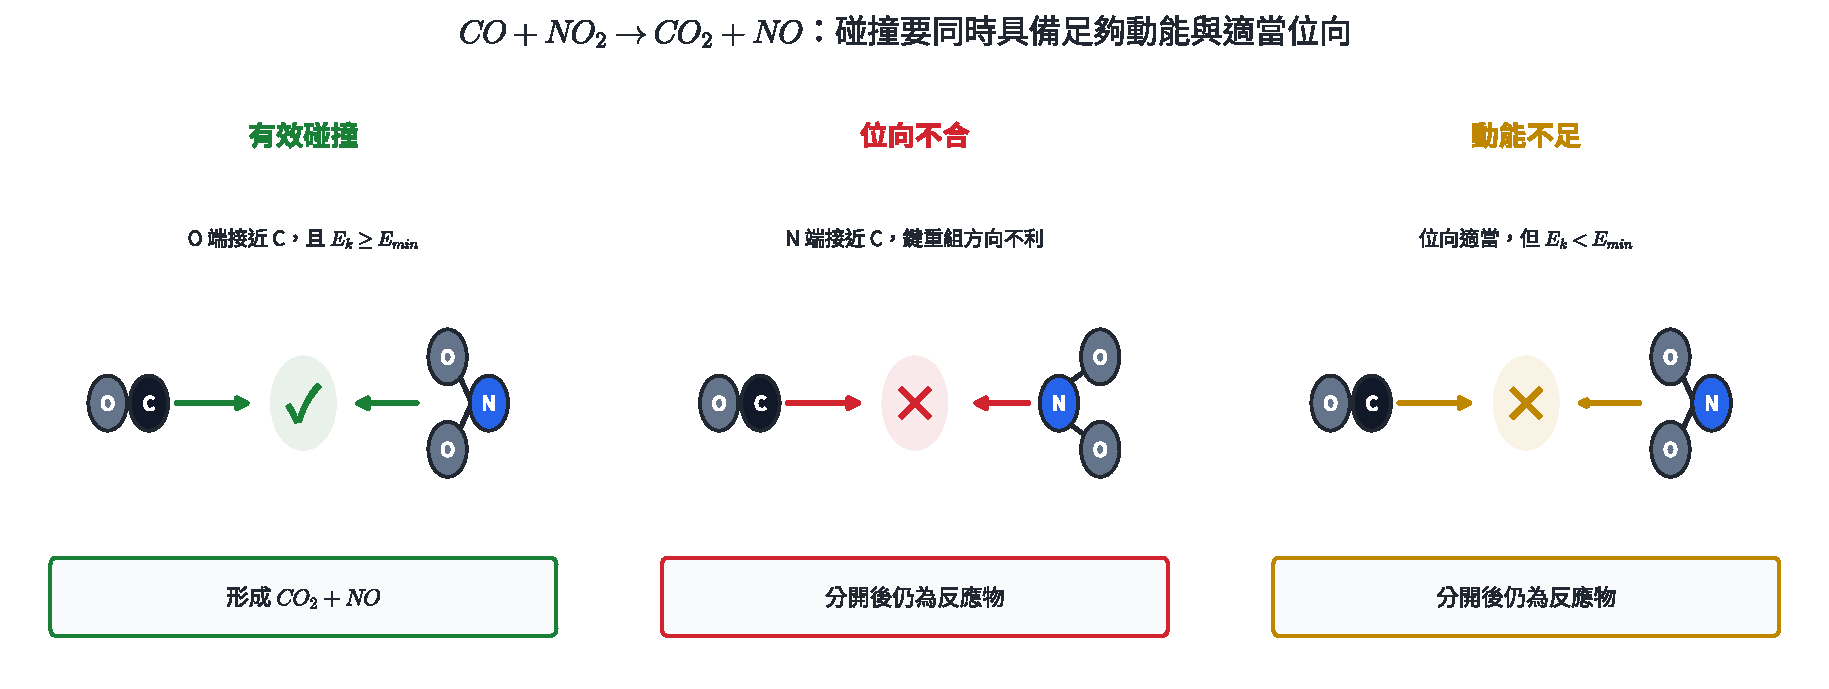
\includegraphics[width=0.99\linewidth,height=\textheight,keepaspectratio,alt={圖 5｜對 CO+NO\_2\textbackslash rightarrow CO\_2+NO 而言，CO 的 C 端接近 NO\_2 的 O 端，並有足夠碰撞動能時，才能完成 O 原子轉移。}]{assets/選化II-3-有效碰撞的能量與位向.pdf}
\caption{圖 5｜對 \(CO+NO_2\rightarrow CO_2+NO\) 而言，CO 的 C 端接近 \(NO_2\) 的 O 端，並有足夠碰撞動能時，才能完成 O 原子轉移。}
\end{figure}

反應速率可用下列架構理解：

\[
\text{有效碰撞頻率}
=\text{總碰撞頻率}
\times\text{能量合格比例}
\times\text{位向合格比例}.
\]

提高濃度常先改變單位時間的總碰撞數；升高溫度同時使碰撞更頻繁，並大幅增加能量合格的粒子比例；催化劑則改變途徑，使能量低限降低。

\begin{HandoutWorkedExample}

\subsection{示範 7｜以碰撞條件解釋三種結果}\label{ux793aux7bc4-7ux4ee5ux78b0ux649eux689dux4ef6ux89e3ux91cbux4e09ux7a2eux7d50ux679c}

對 \(CO+NO_2\rightarrow CO_2+NO\) 而言，比較三次碰撞：

\begin{itemize}
\tightlist
\item
  甲：CO 的 C 端接近 \(NO_2\) 的 O 端，\(E_k>E_{min}\)。
\item
  乙：CO 的 C 端接近 \(NO_2\) 的 N 端，\(E_k>E_{min}\)。
\item
  丙：CO 的 C 端接近 \(NO_2\) 的 O 端，\(E_k<E_{min}\)。
\end{itemize}

甲兼具適當位向與足夠能量，可形成活化複合體並向產物方向發展。乙的能量合格，但原子排列不利於 O 原子轉移；丙的位向合格，但系統無法到達能障頂端。因此乙、丙碰撞後皆回到反應物。

\end{HandoutWorkedExample}

\subsection{2.2 粒子動能分布、活化複合體與活化能}\label{ux7c92ux5b50ux52d5ux80fdux5206ux5e03ux6d3bux5316ux8907ux5408ux9ad4ux8207ux6d3bux5316ux80fd}

固定溫度下，粒子動能呈連續分布；曲線下總面積表示全部粒子。曲線右側 \(E\ge E_a\) 的面積代表能量達到低限的粒子比例。

\begin{figure}
\centering
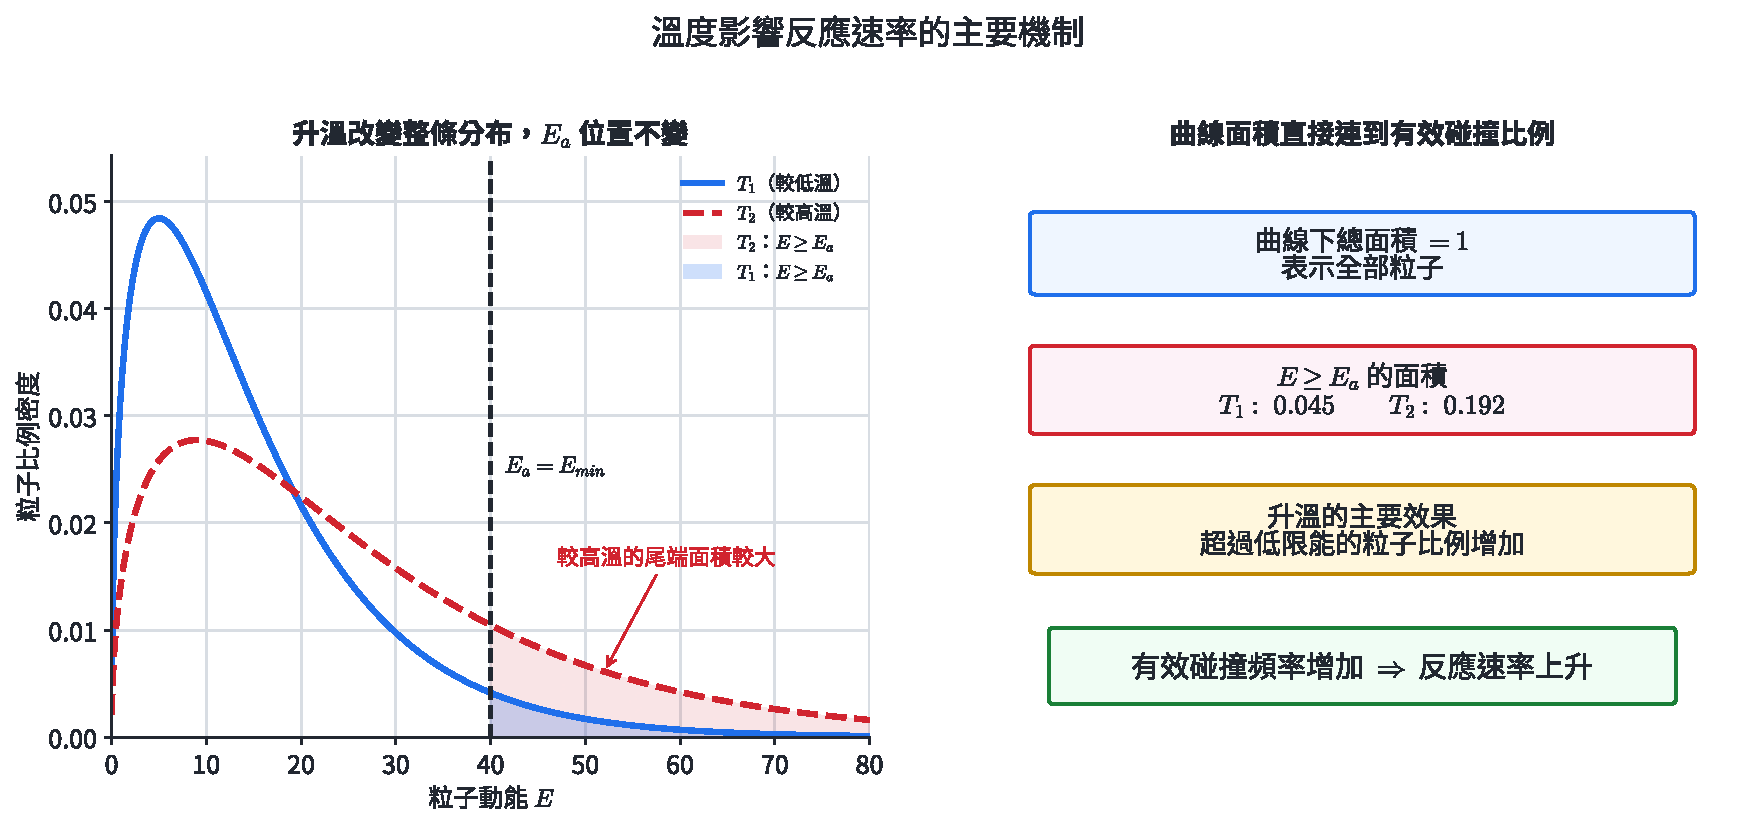
\includegraphics[width=0.98\linewidth,height=\textheight,keepaspectratio,alt={圖 6｜升溫後分布變寬、峰值下降且向高能側移動；固定途徑的 E\_a 位置不變，右側面積增加。}]{assets/選化II-3-粒子動能分布與溫度.pdf}
\caption{圖 6｜升溫後分布變寬、峰值下降且向高能側移動；固定途徑的 \(E_a\) 位置不變，右側面積增加。}
\end{figure}

反應物在轉換為產物的瞬間，形成鍵正在斷裂與形成的高能排列，稱為\textbf{活化複合體}或過渡狀態。由反應物能量上升到該能障頂端所需的能量稱為\textbf{正反應活化能 \(E_a\)}；由產物上升到同一頂端所需能量為\textbf{逆反應活化能 \(E_a'\)}。

\begin{figure}
\centering
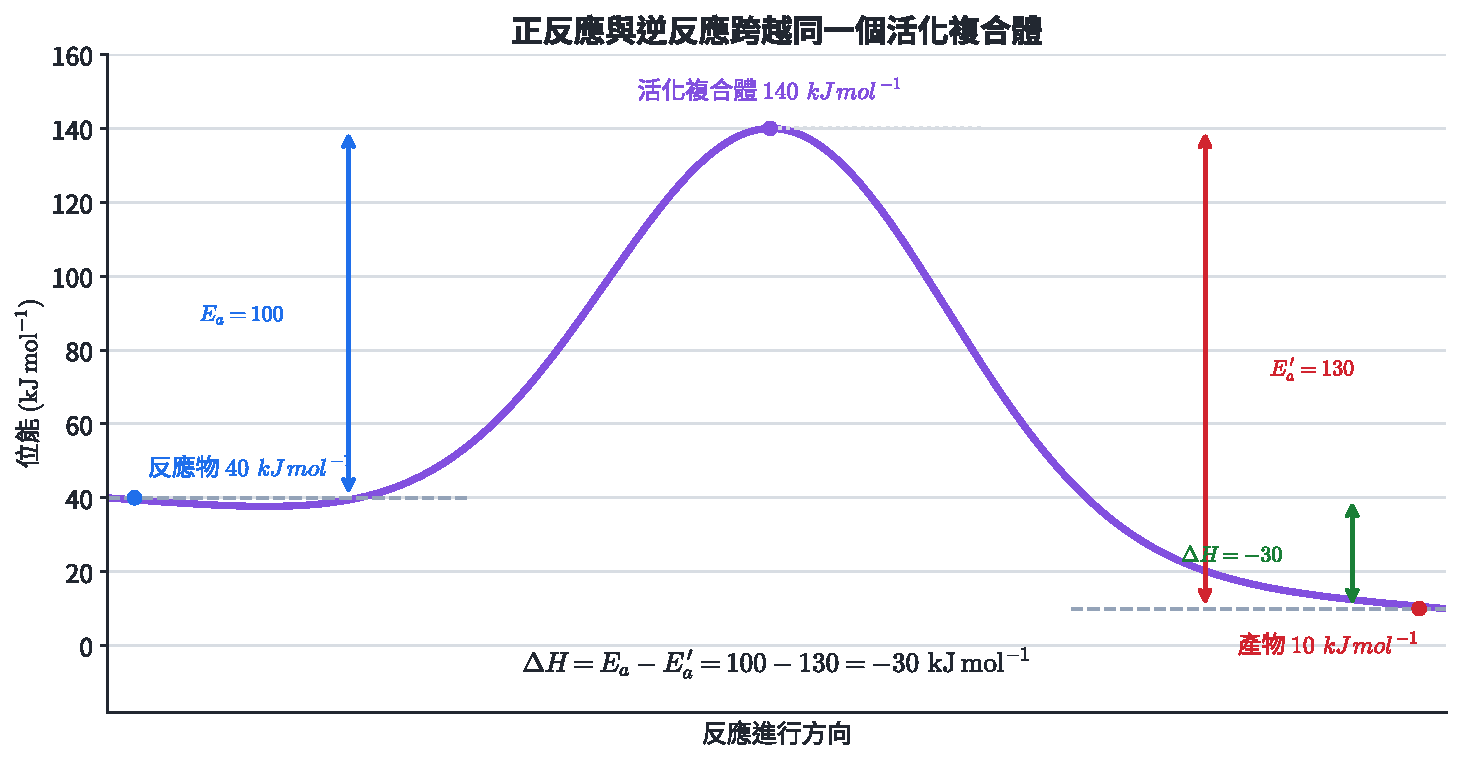
\includegraphics[width=0.92\linewidth,height=\textheight,keepaspectratio,alt={圖 7｜正反應由 40 上升到 140\textbackslash{} \textbackslash mathrm\{kJ\textbackslash,mol\^{}\{-1\}\}，E\_a=100\textbackslash{} \textbackslash mathrm\{kJ\textbackslash,mol\^{}\{-1\}\}；逆反應由 10 上升到 140，E\_a\textquotesingle=130\textbackslash{} \textbackslash mathrm\{kJ\textbackslash,mol\^{}\{-1\}\}。}]{assets/選化II-3-正逆反應能量圖.pdf}
\caption{圖 7｜正反應由 \(40\) 上升到 \(140\ \mathrm{kJ\,mol^{-1}}\)，\(E_a=100\ \mathrm{kJ\,mol^{-1}}\)；逆反應由 \(10\) 上升到 \(140\)，\(E_a'=130\ \mathrm{kJ\,mol^{-1}}\)。}
\end{figure}

反應熱是產物與反應物的能量差：

\[
\Delta H=H_{\mathrm{products}}-H_{\mathrm{reactants}}.
\]

對同一能障頂端，

\[
E_a=H^{\ddagger}-H_{\mathrm{reactants}},
\qquad
E_a'=H^{\ddagger}-H_{\mathrm{products}},
\]

相減得

\[
\boxed{\Delta H=E_a-E_a'}.
\]

放熱反應的 \(\Delta H<0\)，因此 \(E_a<E_a'\)；吸熱反應的 \(\Delta H>0\)，因此 \(E_a>E_a'\)。反應熱比較初、終態；活化能比較起始態與過渡狀態，兩者分屬不同垂直能量差。

\begin{HandoutWorkedExample}

\subsection{示範 8｜由動能分布資料求能量合格碰撞數}\label{ux793aux7bc4-8ux7531ux52d5ux80fdux5206ux5e03ux8cc7ux6599ux6c42ux80fdux91cfux5408ux683cux78b0ux649eux6578}

某溫度下每秒發生 \(2.0\times10^8\) 次碰撞，其中 \(1.5\%\) 的碰撞能量達到 \(E_a\)；能量合格的碰撞中有 \(20\%\) 位向適當。估計每秒有效碰撞數。

\[
N_{\mathrm{effective}}
=(2.0\times10^8)(0.015)(0.20)
=6.0\times10^5\ \mathrm{s^{-1}}.
\]

若升溫使能量合格比例由 \(1.5\%\) 增至 \(4.5\%\)，其他兩項不變，有效碰撞數將變三倍。這個倍率由曲線右尾面積決定；平均動能只描述分布的中心趨勢。

\end{HandoutWorkedExample}

\begin{HandoutWorkedExample}

\subsection{示範 9｜能量圖的正、逆活化能與反應熱}\label{ux793aux7bc4-9ux80fdux91cfux5716ux7684ux6b63ux9006ux6d3bux5316ux80fdux8207ux53cdux61c9ux71b1}

某反應的反應物、產物與活化複合體能量分別為 \(55\)、\(85\)、\(145\ \mathrm{kJ\,mol^{-1}}\)。

\[
E_a=145-55=90\ \mathrm{kJ\,mol^{-1}},
\]

\[
E_a'=145-85=60\ \mathrm{kJ\,mol^{-1}},
\]

\[
\Delta H=85-55=+30\ \mathrm{kJ\,mol^{-1}}.
\]

正反應為吸熱反應，且 \(E_a-E_a'=90-60=+30\ \mathrm{kJ\,mol^{-1}}\)，與 \(\Delta H\) 一致。

\end{HandoutWorkedExample}

\subsection{2.3 基本步驟、反應機構與速率決定步驟}\label{ux57faux672cux6b65ux9a5fux53cdux61c9ux6a5fux69cbux8207ux901fux7387ux6c7aux5b9aux6b65ux9a5f}

實際反應常由多個微觀事件組成。一次碰撞或重排完成的反應單位稱為\textbf{基本步驟}，全部基本步驟的有序集合稱為\textbf{反應機構}。合理機構至少需同時通過三項檢驗：

\begin{enumerate}
\def\labelenumi{\arabic{enumi}.}
\tightlist
\item
  各步驟相加後得到已知總反應。
\item
  反應中間體、催化劑與反應物種的身分對應正確。
\item
  機構推得的速率定律與實驗一致。
\end{enumerate}

\begin{figure}
\centering
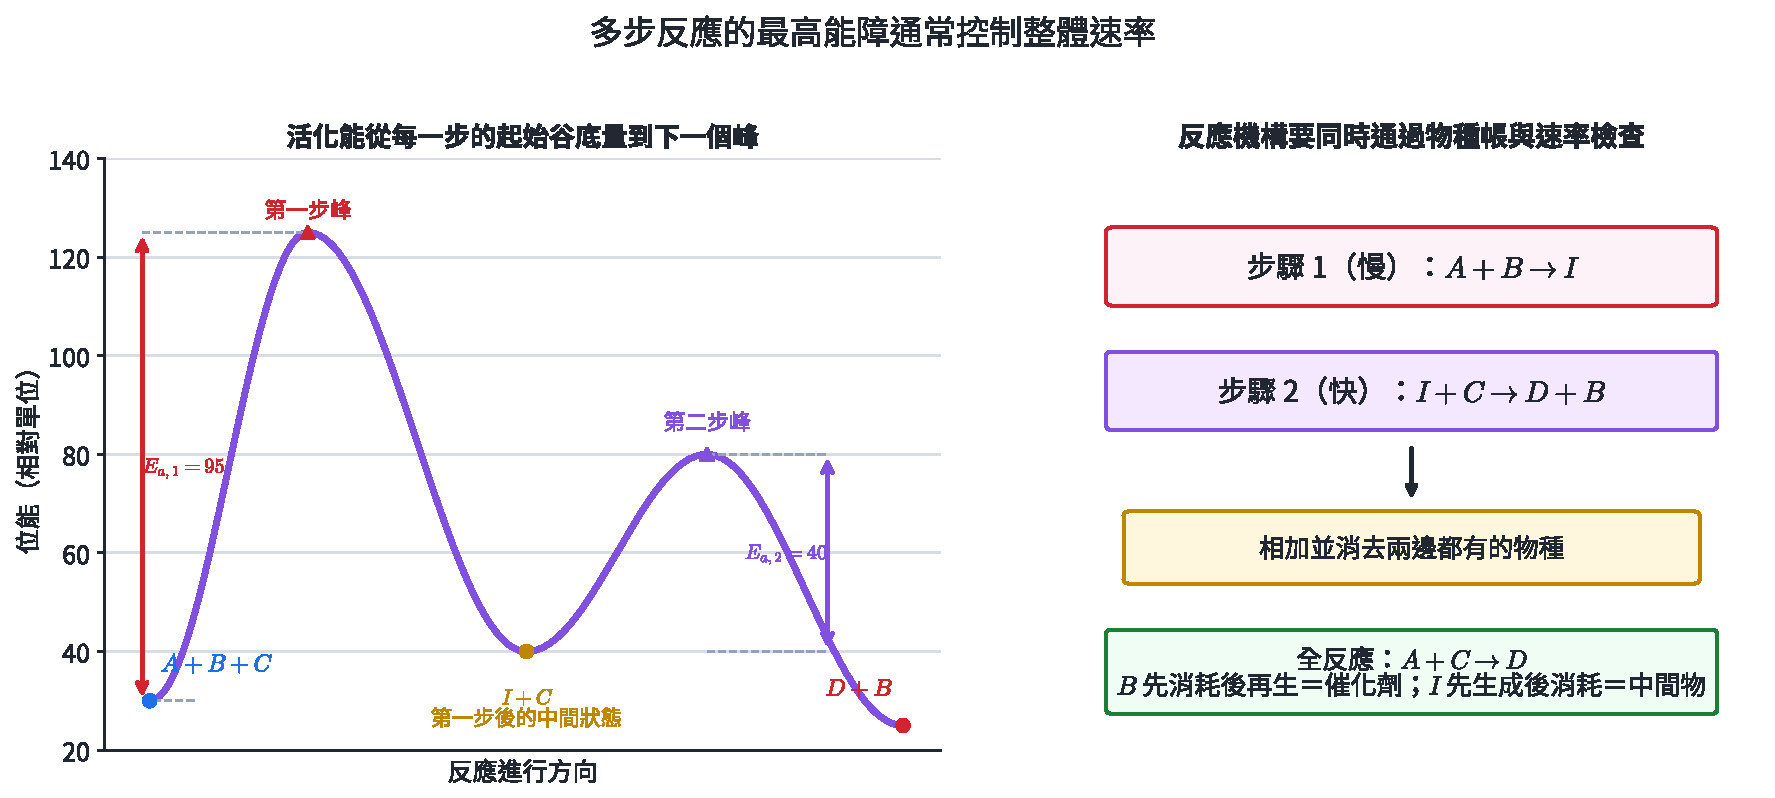
\includegraphics[width=0.98\linewidth,height=\textheight,keepaspectratio,alt={圖 8｜第一步的能障由 A+B+C 能階量到第一個峰，第二步則由中間狀態 I+C 能階量到第二個峰；B 再生，I 消耗。}]{assets/選化II-3-多步反應機構.pdf}
\caption{圖 8｜第一步的能障由 \(A+B+C\) 能階量到第一個峰，第二步則由中間狀態 \(I+C\) 能階量到第二個峰；\(B\) 再生，\(I\) 消耗。}
\end{figure}

圖 8 的機構為

\[
\begin{aligned}
\text{步驟 1（慢）:}&\quad A+B\longrightarrow I,\\
\text{步驟 2（快）:}&\quad I+C\longrightarrow D+B.
\end{aligned}
\]

兩式相加並消去兩邊的 \(B\) 與 \(I\)，得總反應 \(A+C\rightarrow D\)。

\begin{itemize}
\tightlist
\item
  \textbf{中間體 \(I\)}：前一步生成、後一步消耗，不出現於總反應式。
\item
  \textbf{催化劑 \(B\)}：前一步消耗、後一步再生，不出現於總反應式。
\item
  \textbf{速率決定步驟}：對一連串必須依序完成的步驟，最慢的步驟會限制產物形成率。能量圖中需由當前谷底爬升的最高有效能障，常對應此步驟。
\end{itemize}

基本步驟的反應物粒子數稱為\textbf{分子數}：單分子步驟涉及一個粒子，雙分子步驟涉及兩個粒子。三個粒子在正確位向且能量合格的同時碰撞機率很低，所以合理機構常以單分子或雙分子步驟組成。

若圖 8 的第一步是單向慢速基本步驟，則可由此步驟寫出

\[
r=k[A][B].
\]

這也預測：雖然 \(B\) 不出現在總反應式中，其濃度仍可影響速率，因為 \(B\) 實際參與慢步驟。

\begin{HandoutWorkedExample}

\subsection{示範 10｜由基本步驟建立物種帳}\label{ux793aux7bc4-10ux7531ux57faux672cux6b65ux9a5fux5efaux7acbux7269ux7a2eux5e33}

已知機構：

\[
\begin{aligned}
NO_2+NO_2&\longrightarrow NO_3+NO &&\text{（慢）},\\
NO_3+CO&\longrightarrow NO_2+CO_2 &&\text{（快）}.
\end{aligned}
\]

兩式相加，左右同時消去一個 \(NO_3\) 與一個 \(NO_2\)：

\[
NO_2+CO\longrightarrow NO+CO_2.
\]

\(NO_3\) 由第一步生成、第二步消耗，是中間體。\(NO_2\) 的合計結果仍消耗一個，因此是總反應物，同時也參與機構內的再生步驟。慢步驟是雙分子基本步驟，故預測

\[
r=k[NO_2]^2.
\]

若實驗正好得到這個速率律，該機構通過速率檢驗；一致性代表機構可行，後續仍可以用中間體觀測等證據區分其他也符合速率律的機構。

\end{HandoutWorkedExample}

\begin{HandoutWorkedExample}

\subsection{示範 11｜辨認催化劑、中間體與總反應}\label{ux793aux7bc4-11ux8fa8ux8a8dux50acux5316ux5291ux4e2dux9593ux9ad4ux8207ux7e3dux53cdux61c9}

機構為

\[
\begin{aligned}
X+ClO^-&\longrightarrow XO+Cl^-,\\
XO+O_3&\longrightarrow X+2O_2.
\end{aligned}
\]

相加並消去 \(X\) 與 \(XO\)：

\[
ClO^-+O_3\longrightarrow Cl^-+2O_2.
\]

\(X\) 在第一步消耗、第二步再生，是催化劑；\(XO\) 在第一步生成、第二步消耗，是中間體。物種身分由「在機構中的出現順序」決定，不由單一步驟的左右位置決定。

\end{HandoutWorkedExample}

\begin{HandoutWorkedExample}

\subsection{示範 12｜用實驗速率律篩選機構}\label{ux793aux7bc4-12ux7528ux5be6ux9a57ux901fux7387ux5f8bux7be9ux9078ux6a5fux69cb}

總反應為 \(2A+B\rightarrow P\)，實驗速率律是 \(r=k[A][B]\)。考慮兩個候選機構的慢步驟：

\begin{itemize}
\tightlist
\item
  機構甲：\(A+B\rightarrow I\)（慢）。
\item
  機構乙：\(A+A\rightarrow J\)（慢）。
\end{itemize}

甲的慢步驟預測 \(r=k[A][B]\)，與實驗一致。乙的慢步驟預測 \(r=k[A]^2\)，無法表示實驗中 \(B\) 的一級效應。因此這組證據支持機構甲。完整甲機構仍需有後續步驟使各式相加成 \(2A+B\rightarrow P\)。

\end{HandoutWorkedExample}

\subsection{2.4 機構模型的實際用途}\label{ux6a5fux69cbux6a21ux578bux7684ux5be6ux969bux7528ux9014}

工業上改良反應時，單純增加所有反應物濃度常伴隨壓力、副反應與安全成本。找出速率決定步驟後，可把設計焦點放在相關物種濃度、中間體穩定性或催化途徑。大氣化學也使用機構追蹤自由基連鎖反應，來解釋臭氧形成與分解。

\subsection{練習 2}\label{ux7df4ux7fd2-2}

\begin{enumerate}
\def\labelenumi{\arabic{enumi}.}
\tightlist
\item
  某反應每秒發生 \(5.0\times10^7\) 次碰撞，能量合格比例為 \(4.0\%\)，位向合格比例為 \(15\%\)。估計每秒有效碰撞數。
\item
  同一反應在 \(T_1\) 與 \(T_2\) 的動能分布曲線下總面積相等；\(T_2\) 曲線較寬、峰值較低，且 \(E\ge E_a\) 的面積較大。判斷何者溫度較高，並連結到速率常數。
\item
  某反應的 \(H_R=25\)、\(H_P=70\)、\(H^{\ddagger}=125\ \mathrm{kJ\,mol^{-1}}\)。求 \(E_a\)、\(E_a'\) 與 \(\Delta H\)，並判斷吸放熱。
\item
  一個兩步反應能量圖的反應物能量為 \(20\)，第一峰為 \(105\)，中間谷為 \(60\)，第二峰為 \(120\)，產物為 \(10\ \mathrm{kJ\,mol^{-1}}\)。比較兩步的正向活化能，並指出較可能的速率決定步驟。
\item
  已知機構：\(A+Q\rightarrow I\)，\(I+B\rightarrow P+Q\)。寫出總反應，並辨認 \(Q\) 與 \(I\) 的身分。
\item
  總反應為 \(A+2B\rightarrow P\)，實驗得 \(r=k[A][B]\)。某機構的第一步是慢速基本步驟 \(A+B\rightarrow I\)，第二步是快速步驟 \(I+B\rightarrow P\)。說明此機構如何同時通過物種帳與速率定律檢驗。
\end{enumerate}

\subsection{練習 2 解析}\label{ux7df4ux7fd2-2-ux89e3ux6790}

\begin{enumerate}
\def\labelenumi{\arabic{enumi}.}
\item
  有效碰撞數為

  \[
  N_{\mathrm{effective}}
  =(5.0\times10^7)(0.040)(0.15)
  =3.0\times10^5\ \mathrm{s^{-1}}.
  \]
\item
  \(T_2\) 較高。兩曲線下總面積都是全部粒子；\(T_2\) 在 \(E_a\) 右側的面積較大，表示能量合格比例較高，有效碰撞頻率與 \(k\) 較大。
\item
  依能階定義計算：

  \[
  E_a=125-25=100\ \mathrm{kJ\,mol^{-1}},
  \]

  \[
  E_a'=125-70=55\ \mathrm{kJ\,mol^{-1}},
  \]

  \[
  \Delta H=70-25=+45\ \mathrm{kJ\,mol^{-1}}.
  \]

  \(\Delta H>0\)，正反應吸熱，並滿足 \(E_a-E_a'=45\ \mathrm{kJ\,mol^{-1}}\)。
\item
  第一步由 \(20\) 上升到 \(105\)，\(E_{a,1}=85\ \mathrm{kJ\,mol^{-1}}\)；第二步由中間谷 \(60\) 上升到 \(120\)，\(E_{a,2}=60\ \mathrm{kJ\,mol^{-1}}\)。在其他微觀因素相近時，第一步能障較高，較可能是速率決定步驟。
\item
  相加後消去 \(Q\) 與 \(I\)，總反應為 \(A+B\rightarrow P\)。\(Q\) 先消耗後再生，是催化劑；\(I\) 先生成後消耗，是中間體。
\item
  兩步相加時 \(I\) 左右消去，得 \(A+2B\rightarrow P\)，符合總反應。慢步驟為 \(A+B\rightarrow I\)，作為雙分子基本步驟預測 \(r=k[A][B]\)，與實驗一致。
\end{enumerate}

\section{3. 影響反應速率的因素}\label{ux5f71ux97ffux53cdux61c9ux901fux7387ux7684ux56e0ux7d20}

速率改變的直接實驗指標是濃度---時間曲線的斜率或初速率。不同操作可以透過三條微觀路徑發生作用：改變碰撞頻率、改變能量合格的粒子比例，或改變反應途徑與能障。

\subsection{3.1 反應物本質}\label{ux53cdux61c9ux7269ux672cux8cea}

反應物本質決定斷鍵、成鍵、電荷吸引、粒子位向與機構的條件。在相同濃度、溫度與物理狀態下，常見趨勢包括：

\begin{itemize}
\tightlist
\item
  溶液中離子間的快速沉殿或酸鹼中和，可在粒子接觸後迅速完成電荷重排。
\item
  需斷裂強共價鍵、經過複雜位向或多步機構的反應，常有較大能障或較小位向合格比例。
\item
  活潑金屬與酸的速率差異，來自金屬失電子與表面狀態的差異。金屬氧化膜可以阻隔反應物，使實驗結果同時受本質與表面條件影響。
\end{itemize}

有效的本質比較需指定反應、介質、濃度、溫度與相態；常見的快速離子反應是在這些條件相當下的模型趨勢。

\begin{HandoutWorkedExample}

\subsection{示範 13｜用粒子層次比較兩種反應}\label{ux793aux7bc4-13ux7528ux7c92ux5b50ux5c64ux6b21ux6bd4ux8f03ux5169ux7a2eux53cdux61c9}

比較等濃度 \(AgNO_3(aq)\) 與 \(NaCl(aq)\) 混合形成 \(AgCl(s)\)，以及乙酸乙酯在室溫水中水解。

沉殿反應的核心粒子式為

\[
Ag^+(aq)+Cl^-(aq)\longrightarrow AgCl(s).
\]

異號離子在溶液中相遇後可迅速進入晶格。酯類水解涉及共價鍵的斷裂與形成，並受親核攻擊位向與多步機構限制。在題述條件下，\(AgCl\) 沉殿通常更快出現。此比較的直接依據是粒子間作用與機構差異。

\end{HandoutWorkedExample}

\subsection{3.2 濃度、氣體分壓與接觸面積}\label{ux6fc3ux5ea6ux6c23ux9ad4ux5206ux58d3ux8207ux63a5ux89f8ux9762ux7a4d}

在液相或氣相的勻相反應中，單位體積的反應物粒子數增加，總碰撞頻率通常增加。定量倍率由實驗速率律的濃度指數決定。對氣體而言，固定溫度下提高某反應物分壓，等價於提高該氣體的單位體積粒子數。

在固---液、固---氣等不勻相反應中，反應主要在界面發生。相同質量的固體切成較小粒徑後，總表面積增加，可同時接觸的反應位點也增加。

\begin{figure}
\centering
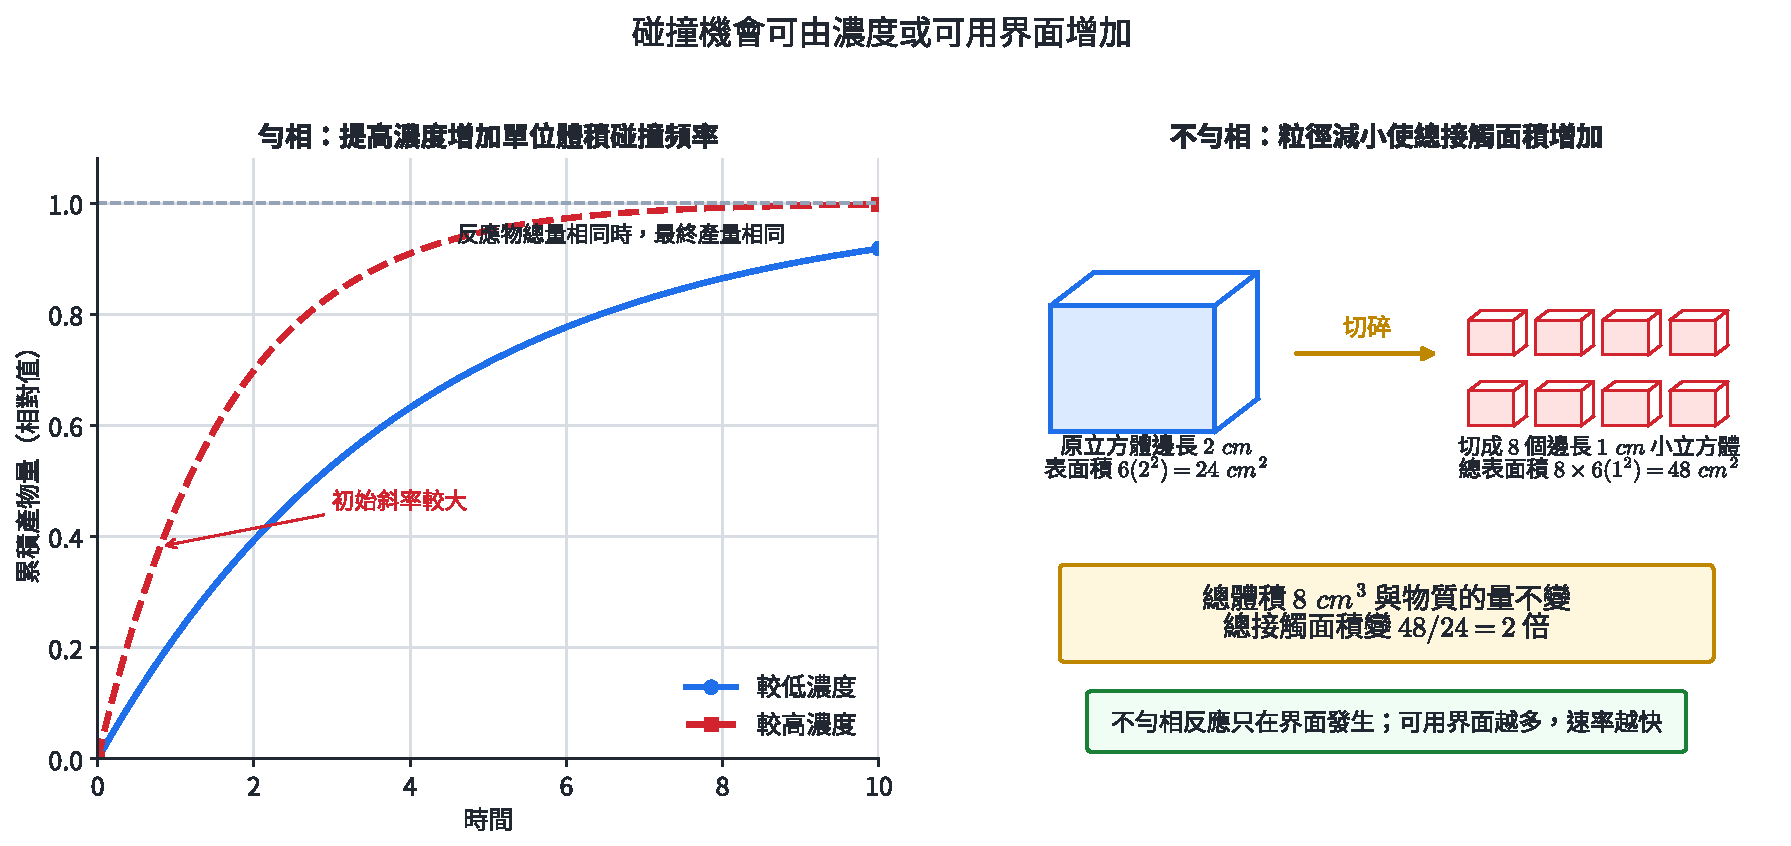
\includegraphics[width=0.99\linewidth,height=\textheight,keepaspectratio,alt={圖 9｜左圖的較高濃度曲線初始斜率較大；右圖把邊長 2\textbackslash{} \textbackslash mathrm\{cm\} 立方體切為 8 個邊長 1\textbackslash{} \textbackslash mathrm\{cm\} 立方體，總表面積由 24 增為 48\textbackslash{} \textbackslash mathrm\{cm\^{}2\}。}]{assets/選化II-3-濃度與接觸面積.pdf}
\caption{圖 9｜左圖的較高濃度曲線初始斜率較大；右圖把邊長 \(2\ \mathrm{cm}\) 立方體切為 \(8\) 個邊長 \(1\ \mathrm{cm}\) 立方體，總表面積由 \(24\) 增為 \(48\ \mathrm{cm^2}\)。}
\end{figure}

當兩組實驗的反應物總莫耳數相同，改變濃度或粒徑可以改變「到達指定轉化率所需時間」，但受限反應物決定的理論最終產量相同。速率與產量是不同的觀測軸。

\begin{HandoutWorkedExample}

\subsection{示範 14｜濃度操作的定量倍率}\label{ux793aux7bc4-14ux6fc3ux5ea6ux64cdux4f5cux7684ux5b9aux91cfux500dux7387}

反應速率律為 \(r=k[A]^{1/2}[B]^2\)。將 \([A]\) 增為四倍、\([B]\) 降為一半，其他條件固定。

\[
\frac{r'}{r}=4^{1/2}\left(\frac12\right)^2
=2\times\frac14=\frac12.
\]

新速率為原速率的 \(0.50\) 倍。碰撞頻率的定性描述可以說明趨勢；此題的精確倍率來自速率定律。

\end{HandoutWorkedExample}

\begin{HandoutWorkedExample}

\subsection{示範 15｜粒徑與總表面積}\label{ux793aux7bc4-15ux7c92ux5f91ux8207ux7e3dux8868ux9762ux7a4d}

一個邊長 \(3.0\ \mathrm{cm}\) 的立方體固體，切成邊長 \(0.50\ \mathrm{cm}\) 的小立方體。計算切割前後總表面積倍率。

原立方體表面積為

\[
S_0=6(3.0)^2=54\ \mathrm{cm^2}.
\]

每邊切成 \(3.0/0.50=6\) 份，共有 \(6^3=216\) 個小立方體。

\[
S=216\times6(0.50)^2=324\ \mathrm{cm^2}.
\]

所以 \(S/S_0=324/54=6.0\)。若表面的活性位點密度與傳質條件相近，可用界面增加解釋反應加快。粉塵與空氣混合時的極大界面，也是粉塵爆燃危害的核心來源。

\end{HandoutWorkedExample}

\subsection{3.3 溫度}\label{ux6eabux5ea6}

升溫使粒子平均動能增加、碰撞頻率略增，更重要的是動能分布中 \(E\ge E_a\) 的面積顯著增加。在機構不變的溫度範圍內，溫度上升使速率常數 \(k\) 增加；精確倍率由該反應在各溫度的速率資料決定。食品冷藏使腐壞反應與微生物酵素速率降低；化學品儲存溫度上限則用來控制分解、聚合或放熱反應的加速。

\begin{HandoutWorkedExample}

\subsection{\texorpdfstring{示範 16｜由兩溫度速率資料比較 \(k\)}{示範 16｜由兩溫度速率資料比較 k}}\label{ux793aux7bc4-16ux7531ux5169ux6eabux5ea6ux901fux7387ux8cc7ux6599ux6bd4ux8f03-k}

某反應的速率律為 \(r=k[A]\)。在 \(298\ \mathrm K\) 與 \(318\ \mathrm K\) 下，使用相同 \([A]_0=0.200\ \mathrm M\) 測得初速率分別為 \(2.40\times10^{-3}\) 與 \(8.55\times10^{-3}\ \mathrm{M\,s^{-1}}\)。

\[
k_{298}=\frac{2.40\times10^{-3}}{0.200}
=1.20\times10^{-2}\ \mathrm{s^{-1}},
\]

\[
k_{318}=\frac{8.55\times10^{-3}}{0.200}
=4.28\times10^{-2}\ \mathrm{s^{-1}}.
\]

\[
\frac{k_{318}}{k_{298}}
=\frac{4.28\times10^{-2}}{1.20\times10^{-2}}
=3.56.
\]

在此濃度下初速率也增為 \(3.56\) 倍。圖 6 提供機制解釋：較高溫度使 \(E\ge E_a\) 的粒子比例增加；精確倍率由實驗速率得到。

\end{HandoutWorkedExample}

\subsection{3.4 催化劑與催化反應}\label{ux50acux5316ux5291ux8207ux50acux5316ux53cdux61c9}

\textbf{催化劑}參與反應機構，提供另一條較低活化能的途徑，並在後續步驟再生。在同一溫度下，較低 \(E_a\) 使動能合格粒子比例增加，故 \(k\) 與反應速率增加。

\begin{figure}
\centering
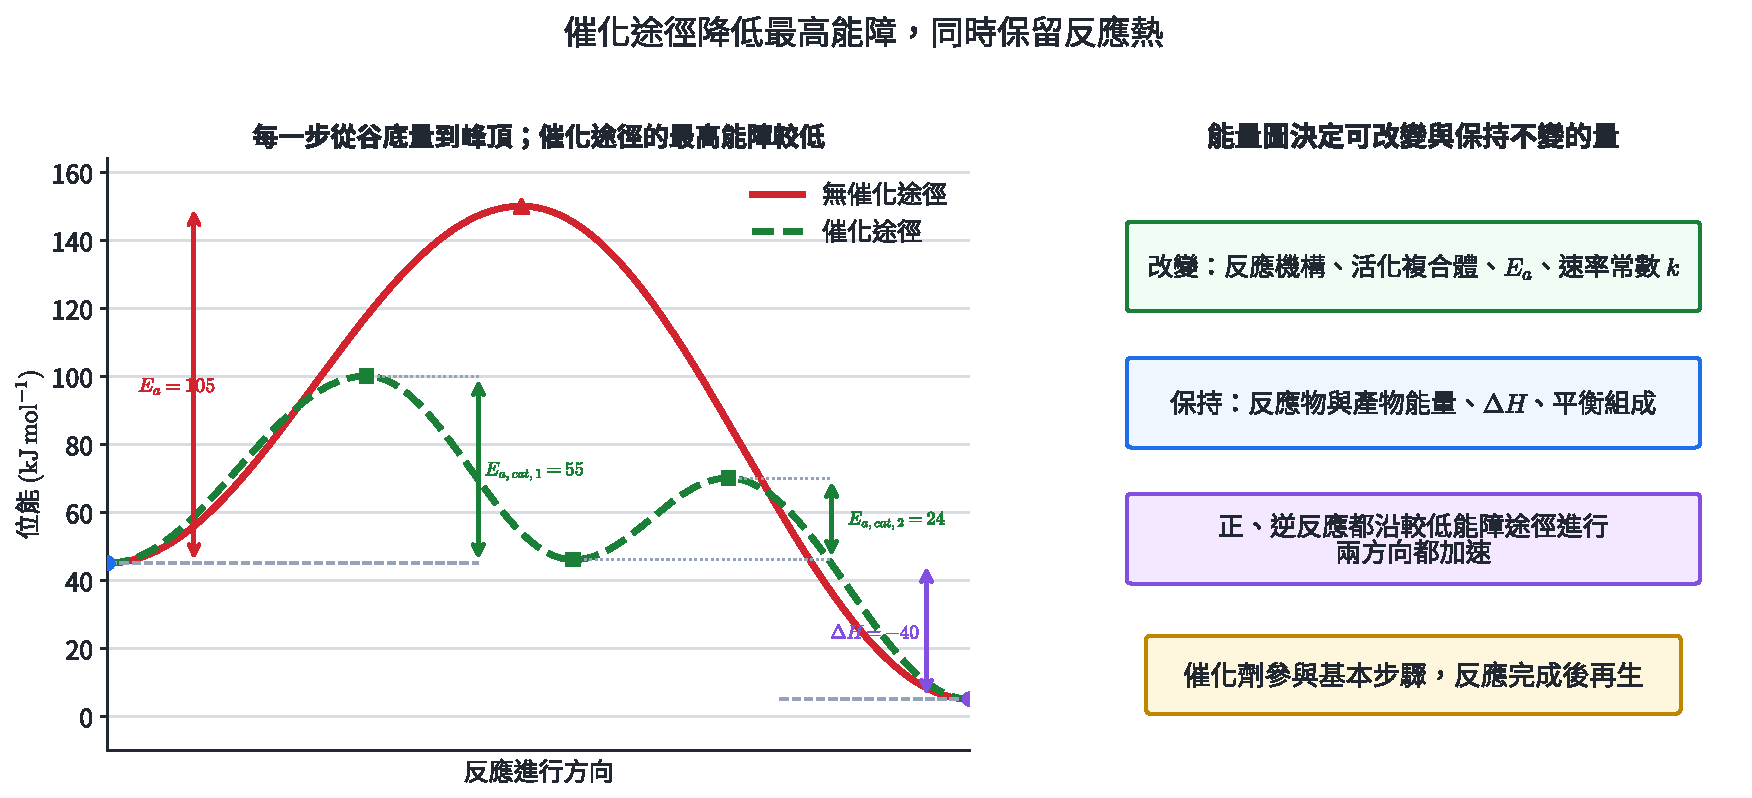
\includegraphics[width=0.97\linewidth,height=\textheight,keepaspectratio,alt={圖 10｜無催化途徑的能障為 105\textbackslash{} \textbackslash mathrm\{kJ\textbackslash,mol\^{}\{-1\}\}；催化途徑兩步分別由當步起始能階量到峰頂，能障為 55 與 24\textbackslash{} \textbackslash mathrm\{kJ\textbackslash,mol\^{}\{-1\}\}。兩途徑的 \textbackslash Delta H=-40\textbackslash{} \textbackslash mathrm\{kJ\textbackslash,mol\^{}\{-1\}\} 相同。}]{assets/選化II-3-催化途徑與反應熱.pdf}
\caption{圖 10｜無催化途徑的能障為 \(105\ \mathrm{kJ\,mol^{-1}}\)；催化途徑兩步分別由當步起始能階量到峰頂，能障為 \(55\) 與 \(24\ \mathrm{kJ\,mol^{-1}}\)。兩途徑的 \(\Delta H=-40\ \mathrm{kJ\,mol^{-1}}\) 相同。}
\end{figure}

催化劑改變反應機構、過渡狀態與正逆反應的活化能，同時保持下列量：

\begin{itemize}
\tightlist
\item
  反應物與產物的能量，因此 \(\Delta H\) 不變。
\item
  總反應式與理論產量不變。
\item
  固定溫度下的平衡常數與平衡組成不變。催化劑同時加速正、逆反應，使系統更快到達原本的平衡。
\end{itemize}

催化劑可以與反應物同相，稱為勻相催化；也可以位於不同相的固體表面，稱為非勻相催化。固體觸媒常透過吸附反應物、調整位向與弱化特定鍵結來降低有效能障。酵素是生物催化劑，活性中心提供適當位向與微環境；過高溫度或極端 pH 可改變其三維結構而降低活性。

\begin{HandoutWorkedExample}

\subsection{示範 17｜由能量數據判斷催化效應}\label{ux793aux7bc4-17ux7531ux80fdux91cfux6578ux64daux5224ux65b7ux50acux5316ux6548ux61c9}

某放熱反應的反應物能量為 \(45\)、產物為 \(5\ \mathrm{kJ\,mol^{-1}}\)。無催化途徑的最高過渡狀態為 \(150\)，催化途徑的最高過渡狀態為 \(100\ \mathrm{kJ\,mol^{-1}}\)。

\[
E_{a,\mathrm{uncat}}=150-45=105\ \mathrm{kJ\,mol^{-1}},
\]

\[
E_{a,\mathrm{cat}}=100-45=55\ \mathrm{kJ\,mol^{-1}}.
\]

兩條途徑的反應熱均為

\[
\Delta H=5-45=-40\ \mathrm{kJ\,mol^{-1}}.
\]

催化途徑將正反應最高能障降低 \(50\ \mathrm{kJ\,mol^{-1}}\)，但初、終能階相同，因此放熱量相同。

\end{HandoutWorkedExample}

\subsection{3.5 碘鐘反應：用固定顏色終點比較速率}\label{ux7898ux9418ux53cdux61c9ux7528ux56faux5b9aux984fux8272ux7d42ux9edeux6bd4ux8f03ux901fux7387}

碘鐘反應將一個連續的化學反應轉成容易計時的顏色突變。本實驗混合含 \(KIO_3\) 的溶液 A，以及含 \(NaHSO_3\)、稀硫酸與澱粉的溶液 B。酸性條件下可以用下列模型理解顏色延遲：

\begin{enumerate}
\def\labelenumi{\arabic{enumi}.}
\tightlist
\item
  \(IO_3^-\) 與含硫物種的氧化還原網路形成碘。
\item
  當 \(HSO_3^-\) 尚存在時，新生成的 \(I_2\) 又被還原為 \(I^-\)，溶液維持無色。
\item
  \(HSO_3^-\) 耗盡後，\(I_2\) 開始累積並與澱粉形成深藍色結合體，產生突然可見的終點。
\end{enumerate}

\begin{figure}
\centering
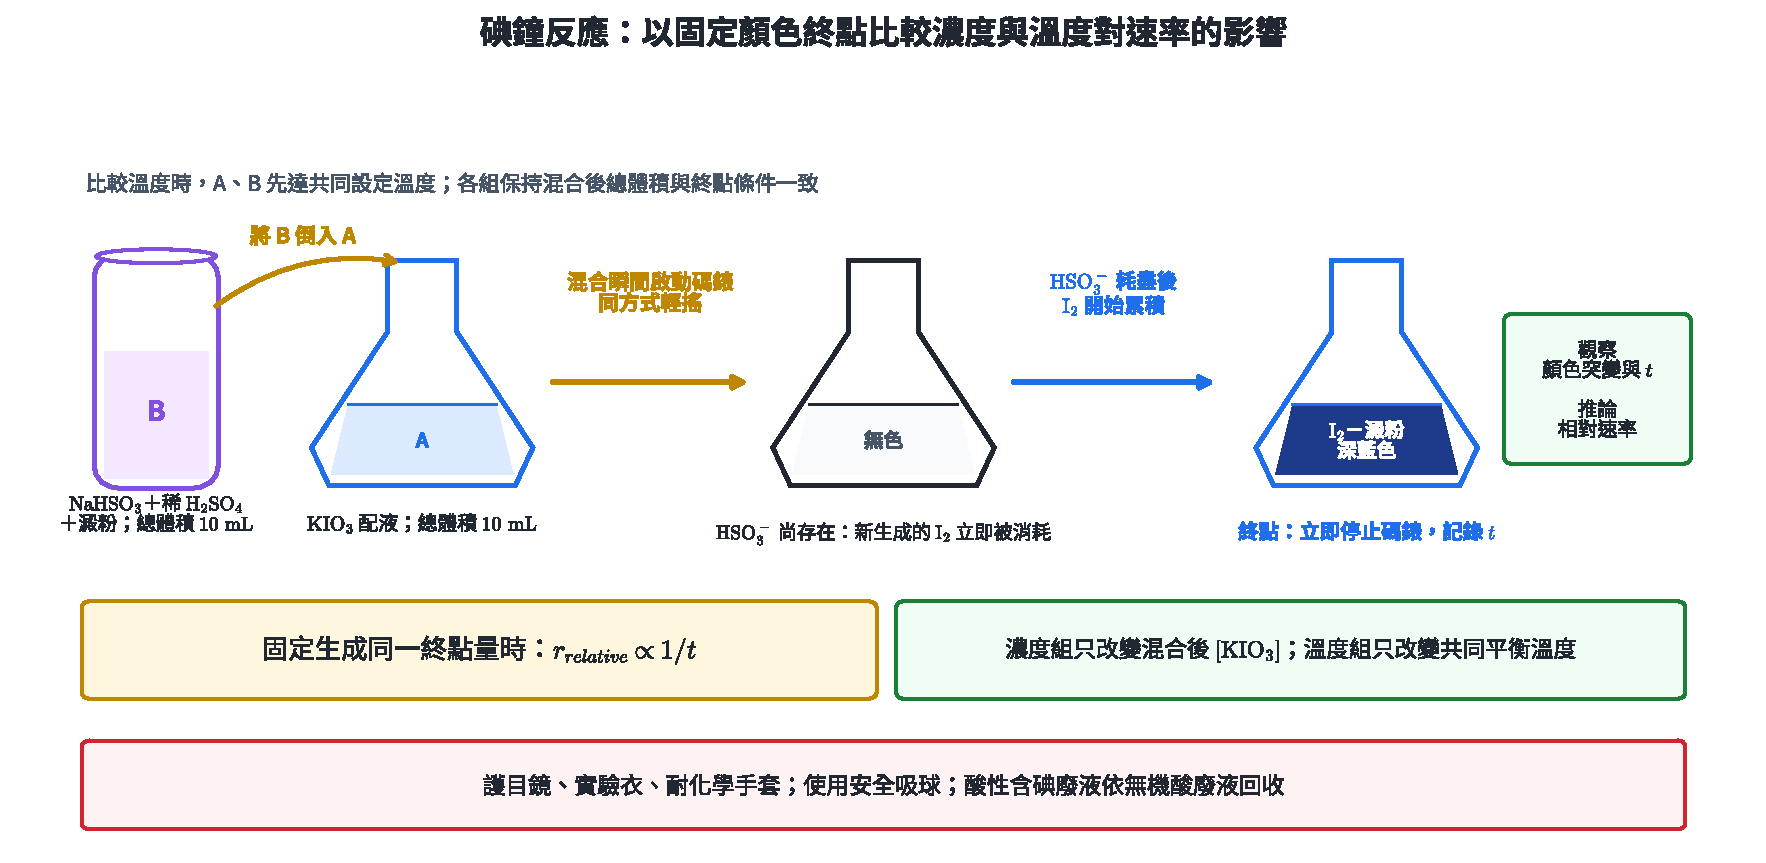
\includegraphics[width=0.99\linewidth,height=\textheight,keepaspectratio,alt={圖 11｜將含 \textbackslash mathrm\{NaHSO\_3\}、稀 \textbackslash mathrm\{H\_2SO\_4\} 與澱粉的 B 溶液由試管倒入裝有 \textbackslash mathrm\{KIO\_3\} A 溶液的錐形瓶，混合瞬間啟動碼錶；\textbackslash mathrm\{HSO\_3\^{}-\} 耗盡後出現深藍色，立即記錄終點時間 t。}]{assets/選化II-3-碘鐘反應裝置與終點.pdf}
\caption{圖 11｜將含 \(\mathrm{NaHSO_3}\)、稀 \(\mathrm{H_2SO_4}\) 與澱粉的 B 溶液由試管倒入裝有 \(\mathrm{KIO_3}\) A 溶液的錐形瓶，混合瞬間啟動碼錶；\(\mathrm{HSO_3^-}\) 耗盡後出現深藍色，立即記錄終點時間 \(t\)。}
\end{figure}

若每次實驗到達終點時都消耗相同量的限量計時試劑，則固定的反應進度 \(\Delta\xi_*\) 滿足

\[
r_{\mathrm{average}}\propto\frac{\Delta\xi_*}{t}
\propto\frac1t.
\]

因此 \(1/t\) 可作為\textbf{相對速率}。這個關係的條件是終點代表的反應量固定；澱粉、\(HSO_3^-\) 的起始量或總體積改變時，終點量也可能改變。

\subsubsection{實驗設計}\label{ux5be6ux9a57ux8a2dux8a08}

\textbf{濃度組}：保持溶液 B 組成、混合後總體積、溫度、攪拌方式與終點判準一致，以蒸餾水與原 \(KIO_3\) 溶液配成不同混合後 \([KIO_3]\)。

\textbf{溫度組}：保持各溶液體積與濃度一致，先將 A、B 分別置於同一恒溫水浴至熱平衡，再混合計時。反應溫度以混合當下的溫度為準，水浴溫度是控制工具。

\textbf{重複與資料}：每個條件至少重複三次，報告平均 \(t\)、\(1/t\) 與散布程度。開始時點、攪拌強度與「持續藍色」的判準需一致。

\begin{figure}
\centering
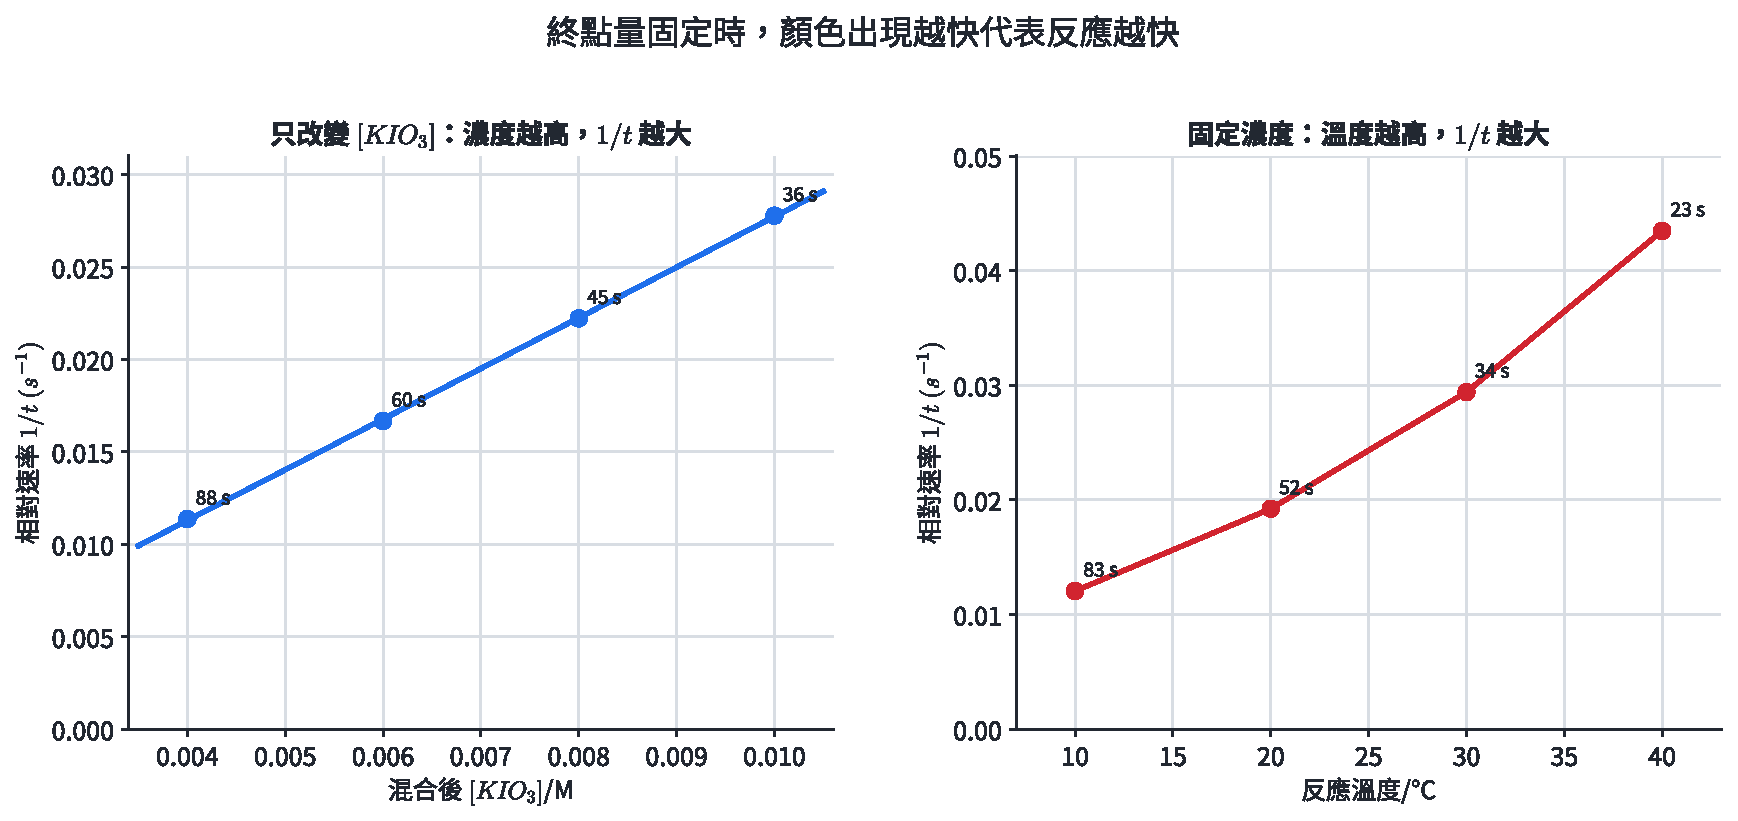
\includegraphics[width=0.97\linewidth,height=\textheight,keepaspectratio,alt={圖 12｜原創資料示範：在終點量固定時，碘酸鉀濃度或溫度增加都使時間 t 縮短、1/t 增加。}]{assets/選化II-3-碘鐘反應資料.pdf}
\caption{圖 12｜原創資料示範：在終點量固定時，碘酸鉀濃度或溫度增加都使時間 \(t\) 縮短、\(1/t\) 增加。}
\end{figure}

\subsubsection{安全、廢棄與證據層次}\label{ux5b89ux5168ux5ee2ux68c4ux8207ux8b49ux64daux5c64ux6b21}

\begin{itemize}
\tightlist
\item
  配戴護目鏡、實驗衣與適當的耐化學手套；以安全吸球操作移液管。
\item
  稀硫酸可造成刺激或腐蝕，碘酸鹽是氧化劑，碘與含碘溶液可刺激並染色。濺觸皮膚或眼睛時以大量流動水沖洗，並依實驗室緊急程序處理。
\item
  反應後溶液含酸性無機鹽與含碘物種，收入實驗室指定的酸性含碘無機廢液容器。
\item
  \textbf{觀察}：混合到持續藍色的時間、溫度、體積與顏色。\textbf{推論}：在終點量一致的條件下，\(1/t\) 較大表示平均反應速率較大。實驗記錄應保留這兩層的區別。
\end{itemize}

\begin{HandoutWorkedExample}

\subsection{示範 18｜由碘鐘資料建立相對速率}\label{ux793aux7bc4-18ux7531ux7898ux9418ux8cc7ux6599ux5efaux7acbux76f8ux5c0dux901fux7387}

在濃度組實驗中，混合後 \([KIO_3]\) 分別為 \(0.0040\)、\(0.0060\)、\(0.0080\)、\(0.0100\ \mathrm M\)，藍色終點時間分別為 \(88\)、\(60\)、\(45\)、\(36\ \mathrm s\)。

{\def\LTcaptype{none} % do not increment counter
\begin{longtable}[]{@{}rrrrr@{}}
\toprule\noalign{}
\([KIO_3]/\mathrm M\) & 0.0040 & 0.0060 & 0.0080 & 0.0100 \\
\midrule\noalign{}
\endhead
\bottomrule\noalign{}
\endlastfoot
\(t/\mathrm s\) & 88 & 60 & 45 & 36 \\
\(1/t/\mathrm{s^{-1}}\) & 0.0114 & 0.0167 & 0.0222 & 0.0278 \\
\end{longtable}
}

當 \([KIO_3]\) 由 \(0.0040\) 增至 \(0.0080\ \mathrm M\)，濃度變兩倍，\(1/t\) 由 \(0.0114\) 增至 \(0.0222\ \mathrm{s^{-1}}\)，約變 \(1.95\) 倍。在本資料範圍內，結果支持相對速率對 \([KIO_3]\) 近似一級。這是由數據得到的實驗級數；與總反應式的係數屬於不同來源。

\end{HandoutWorkedExample}

\subsection{3.6 速率控制的實際用途}\label{ux901fux7387ux63a7ux5236ux7684ux5be6ux969bux7528ux9014}

\begin{itemize}
\tightlist
\item
  \textbf{冷藏與儲存}：降低溫度使食品氧化、香味分解與微生物反應的 \(k\) 降低。
\item
  \textbf{工業反應器}：濃度、壓力、溫度與催化劑同時影響速率；工程設計並需處理散熱、傳質、副反應與爆燃界限。
\item
  \textbf{觸媒轉化器}：固體表面促進 CO、碳氫化合物與氮氧化物轉化；多孔材料提供大表面積，可用界面與催化兩個模型同時解釋。
\item
  \textbf{藥物與酵素}：藥物代謝速率影響作用時間；酵素的活性中心與受質濃度決定生化反應速率。
\end{itemize}

\subsection{練習 3}\label{ux7df4ux7fd2-3}

\begin{enumerate}
\def\labelenumi{\arabic{enumi}.}
\tightlist
\item
  對速率律 \(r=k[A]^2[B]\)，將 \([A]\) 加倍且 \([B]\) 降為原來的 \(1/4\)，溫度不變。求新舊速率比，並說明 \(k\) 的狀態。
\item
  一個邊長 \(4.0\ \mathrm{cm}\) 立方體切成邊長 \(1.0\ \mathrm{cm}\) 的小立方體。求切割前後總表面積與倍率，並指出此變因對不勻相反應的作用。
\item
  某反應在 \(300\ \mathrm K\) 與 \(310\ \mathrm K\) 的速率常數分別為 \(1.80\times10^{-3}\) 與 \(3.91\times10^{-3}\ \mathrm{s^{-1}}\)。求 \(k_{310}/k_{300}\)，並用粒子動能分布解釋趨勢。
\item
  某反應的反應物能量為 \(20\)、產物為 \(50\ \mathrm{kJ\,mol^{-1}}\)。無催化與催化途徑的最高過渡狀態分別為 \(110\) 與 \(75\ \mathrm{kJ\,mol^{-1}}\)。求兩條途徑的正反應 \(E_a\)與 \(\Delta H\)，並說明哪些量改變。
\item
  碘鐘反應中，條件甲的藍色終點時間為 \(72\ \mathrm s\)，條件乙為 \(48\ \mathrm s\)。令兩組的相對速率分別為 \(r_A\)、\(r_B\)；在終點量一致時，求 \(r_B/r_A\)。
\item
  為測試溫度對碘鐘反應的影響，某組將溶液 A 加熱至 \(40^\circ\mathrm C\)，溶液 B 保持 \(20^\circ\mathrm C\)，混合後立即計時，且高溫組使用較少的 B 以配合容器。指出兩個會破壞單一自變因比較的設計，並提出完整修正。
\end{enumerate}

\subsection{練習 3 解析}\label{ux7df4ux7fd2-3-ux89e3ux6790}

\begin{enumerate}
\def\labelenumi{\arabic{enumi}.}
\item
  由速率律計算：

  \[
  \frac{r'}{r}=2^2\left(\frac14\right)=1.
  \]

  新舊速率相同。溫度、催化途徑與介質皆未改變，因此 \(k\) 保持相同。
\item
  原表面積 \(S_0=6(4.0)^2=96\ \mathrm{cm^2}\)。切成 \(4^3=64\) 塊，總表面積 \(S=64\times6(1.0)^2=384\ \mathrm{cm^2}\)，是原來的 \(4.0\) 倍。不勻相反應的可用界面增加，所以在其他條件相近時反應加快。
\item
  速率常數倍率為

  \[
  \frac{k_{310}}{k_{300}}
  =\frac{3.91\times10^{-3}}{1.80\times10^{-3}}
  =2.17.
  \]

  \(310\ \mathrm K\) 的動能分布高能尾較大，\(E\ge E_a\) 的粒子比例較高，因此有效碰撞頻率與 \(k\) 較大。
\item
  無催化 \(E_a=110-20=90\ \mathrm{kJ\,mol^{-1}}\)；催化 \(E_a=75-20=55\ \mathrm{kJ\,mol^{-1}}\)。兩途徑的 \(\Delta H=50-20=+30\ \mathrm{kJ\,mol^{-1}}\)。催化劑改變機構、過渡狀態與 \(E_a\)，而反應物、產物能階與 \(\Delta H\) 保持相同。
\item
  固定終點量時，相對速率與終點時間成反比：

  \[
  \frac{r_B}{r_A}
  =\frac{1/48}{1/72}
  =\frac{72}{48}=1.50.
  \]
\item
  第一，A 與 B 混合後的實際溫度介於兩者起始溫度之間，且混合過程會散熱；修正為將 A、B 同時置於同一恆溫水浴至熱平衡，混合時測實際溫度。第二，改變 B 體積同時改變其混合後濃度、總體積與終點量；修正為各溫度組使用相同批次、濃度與體積的 A、B，並統一攪拌、計時與顏色判準。
\end{enumerate}

\section{4. 核心整理}\label{ux6838ux5fc3ux6574ux7406}

{\def\LTcaptype{none} % do not increment counter
\begin{longtable}[]{@{}
  >{\raggedright\arraybackslash}p{(\linewidth - 4\tabcolsep) * \real{0.3333}}
  >{\raggedright\arraybackslash}p{(\linewidth - 4\tabcolsep) * \real{0.3333}}
  >{\raggedright\arraybackslash}p{(\linewidth - 4\tabcolsep) * \real{0.3333}}@{}}
\toprule\noalign{}
\begin{minipage}[b]{\linewidth}\raggedright
資料或操作
\end{minipage} & \begin{minipage}[b]{\linewidth}\raggedright
直接判讀
\end{minipage} & \begin{minipage}[b]{\linewidth}\raggedright
微觀連結
\end{minipage} \\
\midrule\noalign{}
\endhead
\bottomrule\noalign{}
\endlastfoot
濃度---時間曲線 & 割線給平均速率；切線給瞬時速率 & 反應物逐漸消耗時，有效碰撞頻率常下降 \\
\(aA+bB\rightarrow cC+dD\) & \(r=-\frac1a\frac{\Delta[A]}{\Delta t}=…=\frac1d\frac{\Delta[D]}{\Delta t}\) & 各物種變化依化學計量係數成比 \\
初速率比較 & 由控制變因倍率求 \(m,n\)，再求 \(k\) & 速率律是機構的實驗約束 \\
零級 & \([A]=[A]_0-kt\)；\(t_{1/2}=[A]_0/(2k)\) & 在適用範圍內，反應位點或其他因素使速率不隨 \([A]\) 變化 \\
一級 & \([A]=[A]_0e^{-kt}\)；\(t_{1/2}=0.693/k\) & 每單位時間消耗固定比例 \\
升高濃度或分壓 & 依速率律求倍率 & 單位體積粒子數與碰撞頻率常增加 \\
減小固體粒徑 & 總表面積增加 & 不勻相反應的可用界面增加 \\
升溫 & \(k\) 增加 & \(E\ge E_a\) 的粒子比例顯著增加 \\
加入催化劑 & 正、逆反應都加快；\(\Delta H\) 與平衡組成不變 & 另一條機構具有較低的最高有效能障 \\
碘鐘終點 & 固定終點量下 \(r_{relative}\propto1/t\) & \(HSO_3^-\) 耗盡後，\(I_2\)---澱粉藍色才累積 \\
\end{longtable}
}

\section{5. 章末分層題}\label{ux7ae0ux672bux5206ux5c64ux984c}

\subsection{基礎與資料題 1--12}\label{ux57faux790eux8207ux8cc7ux6599ux984c-112}

\begin{enumerate}
\def\labelenumi{\arabic{enumi}.}
\item
  某反應物 \(A\) 的濃度在 \(t=10.0\ \mathrm s\) 與 \(30.0\ \mathrm s\) 時分別為 \(0.720\) 與 \(0.460\ \mathrm M\)。求此時段 \(A\) 的平均消耗速率，並說明尚需哪種圖形資訊才能求 \(t=20.0\ \mathrm s\) 的瞬時速率。
\item
  對 \(3A+2B\rightarrow4C\)，某時段 \(C\) 的平均生成速率為 \(8.0\times10^{-3}\ \mathrm{M\,min^{-1}}\)。求 \(A\)、\(B\) 的平均消耗速率與歸一化反應速率。
\item
  某反應初速率資料如下。

  {\def\LTcaptype{none} % do not increment counter
  \begin{longtable}[]{@{}
    >{\raggedleft\arraybackslash}p{(\linewidth - 6\tabcolsep) * \real{0.2500}}
    >{\raggedleft\arraybackslash}p{(\linewidth - 6\tabcolsep) * \real{0.2500}}
    >{\raggedleft\arraybackslash}p{(\linewidth - 6\tabcolsep) * \real{0.2500}}
    >{\raggedleft\arraybackslash}p{(\linewidth - 6\tabcolsep) * \real{0.2500}}@{}}
  \toprule\noalign{}
  \begin{minipage}[b]{\linewidth}\raggedleft
  實驗
  \end{minipage} & \begin{minipage}[b]{\linewidth}\raggedleft
  \([A]_0/\mathrm M\)
  \end{minipage} & \begin{minipage}[b]{\linewidth}\raggedleft
  \([B]_0/\mathrm M\)
  \end{minipage} & \begin{minipage}[b]{\linewidth}\raggedleft
  \(r_0/(\mathrm{M\,s^{-1}})\)
  \end{minipage} \\
  \midrule\noalign{}
  \endhead
  \bottomrule\noalign{}
  \endlastfoot
  1 & 0.10 & 0.20 & \(1.2\times10^{-3}\) \\
  2 & 0.20 & 0.20 & \(4.8\times10^{-3}\) \\
  3 & 0.20 & 0.40 & \(4.8\times10^{-3}\) \\
  \end{longtable}
  }

  求速率定律、總級數、\(k\) 與其單位。
\item
  對某單一反應物反應，\([A]\) 對 \(t\) 作圖是斜率 \(-0.015\ \mathrm{M\,min^{-1}}\) 的直線，\([A]_0=0.90\ \mathrm M\)。判斷級數，求 \(k\)、半生期與 \(20.0\ \mathrm{min}\) 後的 \([A]\)。
\item
  某一級反應 \(k=3.50\times10^{-3}\ \mathrm{s^{-1}}\)，\([A]_0=0.600\ \mathrm M\)。求 \(200\ \mathrm s\) 後的 \([A]\) 與半生期。
\item
  對同一反應，升溫後動能分布曲線的峰值降低、高能尾面積增加。用曲線下面積的物理意義說明總粒子數與有效碰撞比例如何變化。
\item
  某反應的 \(E_a=82\)、\(E_a'=117\ \mathrm{kJ\,mol^{-1}}\)。求 \(\Delta H\) 並判斷正反應吸放熱。若反應物能量定為 \(30\ \mathrm{kJ\,mol^{-1}}\)，求產物與活化複合體能量。
\item
  機構如下：

  \[
  \begin{aligned}
  A+X&\longrightarrow I &&\text{（慢）},\\
  I+B&\longrightarrow P+X &&\text{（快）}.
  \end{aligned}
  \]

  寫出總反應、辨認中間體與催化劑，並由慢速基本步驟寫出預測速率律。
\item
  等質量的碳酸鈣一份為大顆粒，另一份研成粉末，分別與等體積、等濃度鹽酸反應。畫出「累積 \(CO_2\) 體積---時間」的相對關係，並比較初斜率與最終體積。
\item
  某反應在 \(290\ \mathrm K\) 與 \(310\ \mathrm K\) 的速率常數分別為 \(1.50\times10^{-3}\) 與 \(5.00\times10^{-3}\ \mathrm{s^{-1}}\)。計算 \(k_{310}/k_{290}\)，並說明濃度條件相同時的初速率倍率。
\item
  對同一反應，無催化途徑 \(E_a=95\ \mathrm{kJ\,mol^{-1}}\)，催化途徑 \(E_a=58\ \mathrm{kJ\,mol^{-1}}\)，\(\Delta H=-22\ \mathrm{kJ\,mol^{-1}}\)。求兩條途徑的逆反應活化能，並說明催化劑對平衡到達時間與平衡組成的影響。
\item
  碘鐘實驗固定終點量，三次重複的終點時間為 \(52.1\)、\(51.7\)、\(70.4\ \mathrm s\)。計算三次平均時間，辨認資料特徵，並提出重測時需固定的三項操作條件。
\end{enumerate}

\subsection{跨節整合題 13--16}\label{ux8de8ux7bc0ux6574ux5408ux984c-1316}

\begin{enumerate}
\def\labelenumi{\arabic{enumi}.}
\setcounter{enumi}{12}
\tightlist
\item
  反應 \(A+B\rightarrow P\) 在 \(298\ \mathrm K\) 的初速率資料為：
\end{enumerate}

{\def\LTcaptype{none} % do not increment counter
\begin{longtable}[]{@{}
  >{\raggedleft\arraybackslash}p{(\linewidth - 6\tabcolsep) * \real{0.2500}}
  >{\raggedleft\arraybackslash}p{(\linewidth - 6\tabcolsep) * \real{0.2500}}
  >{\raggedleft\arraybackslash}p{(\linewidth - 6\tabcolsep) * \real{0.2500}}
  >{\raggedleft\arraybackslash}p{(\linewidth - 6\tabcolsep) * \real{0.2500}}@{}}
\toprule\noalign{}
\begin{minipage}[b]{\linewidth}\raggedleft
實驗
\end{minipage} & \begin{minipage}[b]{\linewidth}\raggedleft
\([A]_0/\mathrm M\)
\end{minipage} & \begin{minipage}[b]{\linewidth}\raggedleft
\([B]_0/\mathrm M\)
\end{minipage} & \begin{minipage}[b]{\linewidth}\raggedleft
\(r_0/(\mathrm{M\,s^{-1}})\)
\end{minipage} \\
\midrule\noalign{}
\endhead
\bottomrule\noalign{}
\endlastfoot
1 & 0.10 & 0.10 & \(2.0\times10^{-4}\) \\
2 & 0.20 & 0.10 & \(4.0\times10^{-4}\) \\
3 & 0.10 & 0.20 & \(8.0\times10^{-4}\) \\
\end{longtable}
}

（a）求速率定律與 \(k_{298}\)。（b）將 \([A]\) 與 \([B]\) 均調為 \(0.15\ \mathrm M\)，求 \(298\ \mathrm K\) 初速率。（c）獨立測量顯示升至 \(318\ \mathrm K\) 後 \(k_{318}=3.74k_{298}\)，計算濃度不變時的初速率，並用動能分布解釋倍率增加。
14. 總反應 \(A+C\rightarrow D\) 的機構為 \(A+B\rightarrow I\)（慢）、\(I+C\rightarrow D+B\)（快）。無催化參考途徑的反應物、過渡狀態、產物能量分別為 \(40\)、\(150\)、\(10\ \mathrm{kJ\,mol^{-1}}\)；含 \(B\) 的兩步途徑最高能量為 \(100\ \mathrm{kJ\,mol^{-1}}\)。（a）建立物種帳並辨認 \(B\)、\(I\)。（b）寫出速率律預測。（c）求兩途徑的正反應 \(E_a\) 與 \(\Delta H\)，並說明 \(B\) 如何改變速率。
15. 碘鐘反應的固定終點實驗得：

{\def\LTcaptype{none} % do not increment counter
\begin{longtable}[]{@{}rrrr@{}}
\toprule\noalign{}
實驗 & \([IO_3^-]_0/\mathrm M\) & \(T/\mathrm K\) & \(t/\mathrm s\) \\
\midrule\noalign{}
\endhead
\bottomrule\noalign{}
\endlastfoot
1 & 0.0040 & 298 & 90 \\
2 & 0.0080 & 298 & 46 \\
3 & 0.0040 & 308 & 55 \\
\end{longtable}
}

（a）以 \(1/t\) 比較實驗 1、2，估計對 \(IO_3^-\) 的級數。（b）比較實驗 1、3 並用動能分布解釋。（c）寫出一個顏色觀察、一個速率推論及四項必須控制的實驗條件。
16. 某固---氣催化反應的速率律在操作範圍內近似 \(r=kP_A\)，反應放熱。工程師考慮同時：將 \(P_A\) 由 \(1.0\) 增至 \(1.8\ \mathrm{bar}\)、將固體觸媒粒徑減半、升高溫度，並加入更有效的催化劑。（a）分別用速率律、接觸面積、動能分布與能量圖解釋四項操作。（b）指出哪些操作改變 \(k\)。（c）說明速率與平衡產率分別由哪些因素決定，並提出兩項放熱系統的工程觀測量。

\section{6. 章末分層題詳解}\label{ux7ae0ux672bux5206ux5c64ux984cux8a73ux89e3}

\subsection{1. 平均與瞬時速率}\label{ux5e73ux5747ux8207ux77acux6642ux901fux7387}

\[
-\frac{\Delta[A]}{\Delta t}
=-\frac{0.460-0.720}{30.0-10.0}
=1.30\times10^{-2}\ \mathrm{M\,s^{-1}}.
\]

這是 \(10.0\) 至 \(30.0\ \mathrm s\) 的割線斜率絕對值。要求 \(20.0\ \mathrm s\) 瞬時速率，需要該時刻附近更密集的濃度資料以建立切線，或直接得到經擬合的 \([A](t)\) 曲線並求當地導數。

\subsection{2. 化學計量速率}\label{ux5316ux5b78ux8a08ux91cfux901fux7387}

由

\[
r=\frac14\frac{\Delta[C]}{\Delta t}
=\frac14(8.0\times10^{-3})
=2.0\times10^{-3}\ \mathrm{M\,min^{-1}}.
\]

因此

\[
-\frac{\Delta[A]}{\Delta t}=3r
=6.0\times10^{-3}\ \mathrm{M\,min^{-1}},
\]

\[
-\frac{\Delta[B]}{\Delta t}=2r
=4.0\times10^{-3}\ \mathrm{M\,min^{-1}}.
\]

三個物種的速率比 \(6.0:4.0:8.0=3:2:4\)，與化學計量係數一致。

\subsection{3. 初速率法}\label{ux521dux901fux7387ux6cd5}

設 \(r=k[A]^m[B]^n\)。實驗 1→2 中 \([A]\) 加倍、\([B]\) 固定，速率變四倍：

\[
4=2^m\Rightarrow m=2.
\]

實驗 2→3 中 \([B]\) 加倍、\([A]\) 固定，速率不變：

\[
1=2^n\Rightarrow n=0.
\]

故

\[
r=k[A]^2,
\qquad N=2.
\]

代入實驗 1：

\[
k=\frac{1.2\times10^{-3}}{(0.10)^2}
=0.12\ \mathrm{M^{-1}\,s^{-1}}.
\]

\(B\) 的零級意味在此實驗範圍內初速率不隨 \([B]\) 變化；\(B\) 仍可以出現在總反應式或機構的其他步驟中。

\subsection{4. 零級反應}\label{ux96f6ux7d1aux53cdux61c9}

\([A]\) 對 \(t\) 是直線，符合零級積分式；斜率是 \(-k\)，故

\[
k=0.015\ \mathrm{M\,min^{-1}}.
\]

\[
t_{1/2}=\frac{[A]_0}{2k}
=\frac{0.90}{2(0.015)}
=30\ \mathrm{min}.
\]

\[
[A]_{20}=0.90-(0.015)(20.0)
=0.60\ \mathrm M.
\]

濃度仍為正，\(20.0\ \mathrm{min}\) 位於該線性模型的物理可用區間內。

\subsection{5. 一級反應}\label{ux4e00ux7d1aux53cdux61c9}

\[
[A]_{200}=0.600e^{-(3.50\times10^{-3})(200)}
=0.600e^{-0.700}
=0.298\ \mathrm M.
\]

\[
t_{1/2}=\frac{0.693}{3.50\times10^{-3}}
=198\ \mathrm s.
\]

\(200\ \mathrm s\) 約為一個半生期，所以剩餘量略少於 \(0.300\ \mathrm M\)，與計算相符。

\subsection{6. 動能分布}\label{ux52d5ux80fdux5206ux5e03}

每條歸一化分布曲線下總面積均為 \(1\)，代表全部粒子，因此升溫不會因曲線峰值下降而使總粒子比例減少。曲線向高能側展寬後，\(E\ge E_a\) 的右尾面積增加，表示能量合格碰撞比例增加。若位向機率與機構不變，有效碰撞頻率上升，因此 \(k\) 與反應速率上升。

\subsection{7. 活化能與反應熱}\label{ux6d3bux5316ux80fdux8207ux53cdux61c9ux71b1}

\[
\Delta H=E_a-E_a'=82-117=-35\ \mathrm{kJ\,mol^{-1}}.
\]

\(\Delta H<0\)，所以正反應放熱。反應物能量為 \(30\ \mathrm{kJ\,mol^{-1}}\)，因此產物能量為

\[
H_P=H_R+\Delta H=30-35=-5\ \mathrm{kJ\,mol^{-1}}.
\]

活化複合體能量為

\[
H^\ddagger=H_R+E_a=30+82=112\ \mathrm{kJ\,mol^{-1}}.
\]

由產物爬至頂端所需能量 \(112-(-5)=117\ \mathrm{kJ\,mol^{-1}}\)，再次驗證 \(E_a'\)。

\subsection{8. 反應機構}\label{ux53cdux61c9ux6a5fux69cb}

兩步相加時，\(I\) 與 \(X\) 在左右各出現一次而消去，得

\[
A+B\longrightarrow P.
\]

\(I\) 先生成、後消耗，是中間體；\(X\) 先消耗、後再生，是催化劑。慢速基本步驟是 \(A+X\rightarrow I\)，故預測

\[
r=k[A][X].
\]

\subsection{9. 接觸面積與氣體產量曲線}\label{ux63a5ux89f8ux9762ux7a4dux8207ux6c23ux9ad4ux7522ux91cfux66f2ux7dda}

等質量 \(CaCO_3\) 且鹽酸量足夠時，兩組的理論 \(CO_2\) 莫耳數相同。粉末的總表面積較大，初始可同時接觸酸的反應位點較多，所以粉末曲線的初斜率較大、更早變平。大顆粒曲線初斜率較小、較晚到達平台。兩曲線最終平台高度相同。

若實驗中鹽酸是限量試劑，最終體積仍由相同的鹽酸莫耳數決定；此判斷需以兩組均完成相同限量反應為前提。

\subsection{\texorpdfstring{10. 溫度對 \(k\) 的影響}{10. 溫度對 k 的影響}}\label{ux6eabux5ea6ux5c0d-k-ux7684ux5f71ux97ff}

\[
\frac{k_{310}}{k_{290}}
=\frac{5.00\times10^{-3}}{1.50\times10^{-3}}
=3.33.
\]

在速率定律的濃度各項都相同時，初速率也增為 \(3.33\) 倍。溫度倍率透過 \(k\) 作用，對應圖 6 中高能尾面積增加。

\subsection{11. 催化途徑的逆活化能}\label{ux50acux5316ux9014ux5f91ux7684ux9006ux6d3bux5316ux80fd}

由 \(\Delta H=E_a-E_a'\)，

\[
E_a'=E_a-\Delta H.
\]

無催化途徑：

\[
E_{a,\mathrm{uncat}}'=95-(-22)=117\ \mathrm{kJ\,mol^{-1}}.
\]

催化途徑：

\[
E_{a,\mathrm{cat}}'=58-(-22)=80\ \mathrm{kJ\,mol^{-1}}.
\]

催化劑同時降低正、逆反應的有效能障，因此縮短達到平衡所需時間。固定溫度下的平衡常數與平衡組成保持相同。

\subsection{12. 碘鐘重複資料}\label{ux7898ux9418ux91cdux8907ux8cc7ux6599}

三次平均為

\[
\bar t=\frac{52.1+51.7+70.4}{3}
=58.1\ \mathrm s.
\]

\(52.1\) 與 \(51.7\ \mathrm s\) 很接近，\(70.4\ \mathrm s\) 則明顯偏離，使平均值遠離前兩次的中心。應保留原始值、查明操作記錄並重測，再根據事先訂定的離群處理規則決定如何匯總。重測時可固定：（1）A、B 混合體積與濃度；（2）混合前熱平衡與混合當下溫度；（3）倒入、啟動碼錶、攪拌與持續藍色判準。

\subsection{13. 速率律、濃度與溫度整合}\label{ux901fux7387ux5f8bux6fc3ux5ea6ux8207ux6eabux5ea6ux6574ux5408}

\textbf{（a）} 設 \(r=k[A]^m[B]^n\)。實驗 1→2，\([A]\) 加倍且速率加倍，故 \(m=1\)。實驗 1→3，\([B]\) 加倍且速率變四倍，故 \(n=2\)。

\[
r=k[A][B]^2.
\]

\[
k_{298}=\frac{2.0\times10^{-4}}{(0.10)(0.10)^2}
=0.200\ \mathrm{M^{-2}\,s^{-1}}.
\]

\textbf{（b）} 在 \(298\ \mathrm K\)，

\[
r_{298}=(0.200)(0.15)(0.15)^2
=6.75\times10^{-4}\ \mathrm{M\,s^{-1}}.
\]

\textbf{（c）} 濃度不變時，速率與 \(k\) 成正比，因此

\[
r_{318}=(3.74)(6.75\times10^{-4})
=2.53\times10^{-3}\ \mathrm{M\,s^{-1}}.
\]

濃度倍率透過 \([A][B]^2\) 作用，溫度倍率透過 \(k\) 作用，兩者在速率律中分工明確。
由圖 6，\(318\ \mathrm K\) 的動能分布高能尾較大，能量達到 \(E_a\) 的粒子比例增加，對應測得 \(k\) 增加。

\subsection{14. 機構、能障與催化整合}\label{ux6a5fux69cbux80fdux969cux8207ux50acux5316ux6574ux5408}

\textbf{（a）} 兩步相加：

\[
\begin{aligned}
A+B&\longrightarrow I,\\
I+C&\longrightarrow D+B,\\ \hline
A+C&\longrightarrow D.
\end{aligned}
\]

\(B\) 先消耗、後再生，是催化劑；\(I\) 先生成、後消耗，是中間體。

\textbf{（b）} 慢速基本步驟為 \(A+B\rightarrow I\)，預測

\[
r=k[A][B].
\]

催化劑 \(B\) 雖在總反應式中消去，仍參與慢步驟並出現於速率律。

\textbf{（c）} 無催化途徑：

\[
E_{a,\mathrm{uncat}}=150-40=110\ \mathrm{kJ\,mol^{-1}}.
\]

含 \(B\) 途徑的最高有效能障：

\[
E_{a,\mathrm{cat}}=100-40=60\ \mathrm{kJ\,mol^{-1}}.
\]

兩途徑的反應熱相同：

\[
\Delta H=10-40=-30\ \mathrm{kJ\,mol^{-1}}.
\]

\(B\) 使最高能障降低 \(50\ \mathrm{kJ\,mol^{-1}}\)，因此在同溫下有更大比例的碰撞能量合格、\(k\) 增加。\(B\) 在後步驟再生，而反應物、產物能階不變。

\subsection{15. 碘鐘資料、溫度與實驗設計整合}\label{ux7898ux9418ux8cc7ux6599ux6eabux5ea6ux8207ux5be6ux9a57ux8a2dux8a08ux6574ux5408}

\textbf{（a）} 終點量固定時 \(r_{relative}\propto1/t\)，因此

\[
\frac{r_2}{r_1}=\frac{1/46}{1/90}
=\frac{90}{46}=1.96.
\]

\([IO_3^-]\) 倍率為 \(0.0080/0.0040=2.00\)。若 \(r\propto[IO_3^-]^m\)，

\[
m=\frac{\ln(1.96)}{\ln2.00}=0.97\approx1.
\]

本資料支持對 \(IO_3^-\) 近似一級。

\textbf{（b）} 實驗 1 與 3 的濃度相同，相對速率比為

\[
\frac{r_3}{r_1}=\frac{90}{55}=1.64.
\]

\(308\ \mathrm K\) 時的動能分布較寬，\(E\ge E_a\) 的右尾面積較大，因此能量合格的碰撞比例、\(k\) 與相對速率都較大。

\textbf{（c）} 觀察：實驗 3 混合後 \(55\ \mathrm s\) 出現持續藍色。推論：在終點量一致時，實驗 3 的平均速率約是實驗 1 的 \(1.64\) 倍。實驗需控制：（1）非自變因反應物的混合後濃度；（2）\(HSO_3^-\) 與澱粉的量，使終點量一致；（3）混合後總體積；（4）攪拌、啟動碼錶與持續藍色的操作判準。比較濃度時溫度也需固定；比較溫度時各溶液濃度需固定。

\subsection{16. 工業速率控制整合}\label{ux5de5ux696dux901fux7387ux63a7ux5236ux6574ux5408}

\textbf{（a）}

\begin{itemize}
\tightlist
\item
  \(P_A\) 由 \(1.0\) 增至 \(1.8\ \mathrm{bar}\)：由 \(r=kP_A\)，在 \(k\) 與觸媒面積固定時，速率增為 \(1.8\) 倍；分壓上升代表單位體積 \(A\) 粒子數增加。
\item
  觸媒粒徑減半：總質量、形狀相似且孔道可用時，總外表面積約增為兩倍；實際效果仍受孔道擴散、壓降與磨耗影響。
\item
  升溫：動能分布中 \(E\ge E_a\) 面積增加，速率常數 \(k\) 增加。
\item
  更有效的催化劑：提供較低最高能障的反應機構，使同溫下的 \(k\) 增加，同時保持反應物與產物能階。
\end{itemize}

\textbf{（b）} 升溫與改用催化劑會改變 \(k\)；\(P_A\) 改變速率律的壓力項；粒徑改變可用位點總數。若 \(k\) 是每單位活性面積的內在常數，粒徑只改變裝置的表觀速率。

\textbf{（c）} 速率屬動力學，平衡產率由熱力學決定。催化劑同時加速正、逆反應，只縮短達平衡的時間。放熱平衡反應升溫時速率加快，平衡組成可朝反應物移動；壓力效應由反應前後氣體莫耳數決定。

放熱系統應連續監測反應床溫度與熱點、冷卻流體進出口溫度、系統壓力與壓降、排放組成，以辨認熱移除失效、速率自加速、觸媒床阻塞與異常轉化。


\end{document}
